% tGISguide.tex
% v3.4 released April 2009

\documentclass[]{tGIS2e}
%\citestyle{tGIS}


\begin{document}

%\doi{10.1080/1365881YYxxxxxxxx}
%\issn{1362-3087} \issnp{1365-8816} \jvol{00} \jnum{00} \jyear{2009} %\jmonth{February}

%\markboth{Taylor \& Francis and I.T. Consultant}{International Journal of Geographical Information Science}

\articletype{RESEARCH ARTICLE}
\title{{\itshape Depicting urban boundaries from a mobility network of spatial interactions: A case study of Great Britain with geo-located Twitter data} }
\maketitle

\begin{abstract}
Existing urban boundaries are usually defined by government agencies for political and administrative purposes.
However, it is not clear whether the boundaries truly reflect people's interactions with the urban space in their intra- and inter-regional activities.
Defining urban boundaries which consider socio-economic relationships and citizen commute patterns is important for many aspects of urban planning.
In this study, we presented a method to redraw urban boundaries based upon human interactions with the physical space.
Specifically, we depicted the urban boundaries of Great Britain using a mobility network of Twitter user spatial interactions that was inferred from over 69 million geo-located Twitter messages.
We redrew the non-administrative anthropographic boundaries in a hierarchical fashion based on different physical movement ranges of users inferred from the collective mobility patterns of Twitter users in Great Britain.
The results of strongly connected urban regions in the form of communities in the network space yield geographically cohesive, non-overlapping urban areas, which provide a clear delineation of the non-administrative anthropographic urban boundaries of Great Britain.
The technique was applied to both national (Great Britain) and municipal scales (the London metropolis).
While our results corresponded well with the administrative boundaries, many unexpected and interesting boundaries were identified.
More importantly, as the depicted urban boundaries exhibited a strong instance of spatial proximity, we further employed a gravity model to connect human mobility research to understand and justify the distance decay effects in shaping the delineated urban boundaries.
This well fitted gravity model explains how geographical distances found in the mobility patterns affect the interaction strength among different non-administrative anthropographic urban areas, which provides a new understanding of the interactions between human activity and urban space.
\newline

\noindent{\bf{Keywords:}} mobility pattern, urban boundary, spatial interaction, spatial network, community structure
\end{abstract}

\section{Introduction}
Official urban boundaries are defined by government agencies for political and administrative purposes.
Urban environments are conceptualized as spaces that are recreated and formed by human activities~\citep{schliephake}.
A fundamental question when using the administrative, ``top-down'', approach to defining urban boundaries is whether the outcome reflects the spatial interactions of humans.
These interactions can take the form of trade, commerce, social connections, and political activity across borders.
Urban boundaries that respect the human interaction space are important to city planning, traffic management and resource allocation~\citep{gao2014, jiang2015,liu2015,long2015}.
Many studies adopt a ``bottom-up'' approach to urban boundary delineation, where the geographic space is partitioned into small units and each unit is represented as a node within a network structure.
A suitable community detection algorithm is applied to partition the network and associated geographic space based on the strength of human interaction among the nodes~\citep{lancichinetti2009}.
Different social and physical human interactions were considered to establish the edges of the network connecting the nodes.
For example, a large set of telephone call records were used to represent the network of human interaction across space to delineate urban boundaries in Great Britain~\citep{ratti2010}.
Extending the previous method to different countries~\citep{sobolevsky2013}, the authors argue that this method yields cohesive geographic divisions that follow the socio-economic boundaries.
While other researchers use social ties of Twitter users to identify cohesive regions for different countries across the world~\citep{kallus2015}, they found evidence for dividing the urban space due to local conflicts and cross-country unifying trends that further support the ``bottom-up" approach to mapping non-administrative anthropographic boundaries.

A common outcome observed in the mentioned studies is that the strongly connected urban regions in the form of communities in the network space yield geographically cohesive areas, in spite of different community detection methods and various forms of social and physical human interactions were used.
A general consensus is that those geographically cohesive areas are instances of the effects on spatial proximity, where the interaction strength between two urban regions decreases as the geographical distance between them increases~\citep{fotheringham1981}.
In particular, spatial proximity is closely related to Tobler's First Law of Geography: ``\textit{everything is related to everything else, but near things are more related than distant things}''~\citep{miller2004}.
While it is perhaps intuitively logical, few research efforts, which seek to quantitatively understand and explain how the spatial interactions shape the forms of connected geographical areas (i.e., urban boundaries), have been carried out. 
One of the major reasons is that geographical distance may affect the interaction strength, it is not an explicitly expressed constraint in the ``virtual'' human interactions, such as social ties or phone call initiation.
In addition, there is a general lack of exploration regarding the linkages between the spatial proximity effects and the characteristics of the underlying spatial interactions. 

In this study, we describe a novel approach to delineating non-administrative anthropographic urban boundaries from a mobility network of physical human spatial interactions.
Specifically, the spatial interactions refer to the actual movements of Twitter users (i.e., the reallocation across the geographical space), which were extracted from more than 69 million Twitter messages from June $1^{st}$ to December $31^{st}$, 2014.
Geo-located Twitter data is proven to be a useful source for studying human mobility patterns at large spatial scales (e.g. the national level)~\citep{hawelka,jurdak2015}.
In addition, Twitter data are not as sensitive to user privacy issues and do not exhibit spatial granularity that is limited to the postal code level~\citep{thiemann}. 
We argue here that by investigating Twitter user mobility patterns, we can provide a different view of non-administrative units based on physical commutes rather than social ties or phone call initiation. 
A unique advantage is that non-administrative anthropographic urban boundaries can be delineated in a hierarchical fashion based upon different ranges of physical movement, which are inferred from the collective mobility patterns of Twitter users in Great Britain. 

We delineated the geography of urban boundaries in Great Britain by imposing a virtual fishnet over the islands of Great Britain.
Twitter user movements were used to establish the connections between the fishnet's cells to form a connectivity network, where each cell acts as a node within the network.
We applied the map equation algorithm~\citep{domenico2015} to partition the network and associate geographic regions.
The map equation algorithm was selected to avoid the inherent resolution problem~\citep{fortunato2007} of the common modularity maximization method~\citep{newman2006}. 
We found that the collective mobility patterns of Twitter users in Great Britain are divided into several distance ranges ranging from short, intra- to inter-city movements with clear distinction points. 
The identification of connected regions at each of these distance ranges yielded hierarchical boundaries of urban spaces in Great Britain.
As the depicted urban boundaries exhibited a strong instance of spatial proximity, we further employed a gravity model to connect human mobility research to understand and justify the distance decay effects in shaping the delineated urban boundaries.
The well fitted gravity model explains how geographical distances found in the mobility patterns affect the interaction strength among different non-administrative anthropographic urban areas. 
Our study provides a first-step in connecting human mobility research with the delineation of non-administrative anthropographic urban boundaries based on Twitter user spatial interaction. 
This provides a new understanding of the interactions between human activities and urban space. 

\section{Background and Related Work}
In real-world geography, urban regions are discrete components in a greater set of regions, with or without physical boundaries separating them~\citep{jiang2015}.
For political and administrative purposes, government agencies define various sets of boundaries to partition the geographical space into spatial units at different scales, for instance: states, counties, census tracts, and electoral districts.
However, the spatial extents of these units often overlap and agglomerate depending how citizens perceive, organize their image of a city, and interact with the urban environments~\citep{lynch1960}.
As connections are made between these units via various human activities crossing boarders, such as social-economic relations and commute patterns of citizens, certain groups of units become more strongly connected than others. The boundaries of the agglomeration of these units are argued to reflect how people naturally interact with their geographical environment, which is important for city planning~\citep{hollenstein2010}, urban growth evaluations~\citep{jiang2015,long2015}, and traffic management~\citep{gao2014}. 

Empirical studies have attempted to delineate such boundaries with different methods and data sets.
In general, the methods from existing literature can be summarized into two classes: spatial clustering and network based approaches.
Spatial-clustering based approaches determine the boundaries based the intensity of geographic locations related to human activities, for instance: locations of social media check-ins~\citep{cranshaw2012,jiang2015,sun2016}, place descriptions from crowd-sourced Web content~\citep{vasardani2013}, and geo-tagged Flickr data~\citep{stefanidis2013,hu2016}.
While notable boundaries of urban areas were identified and delineated, the dynamic connections between different spatial units were neglected in the spatial clustering based approaches, where the results are discrete and independent areas reflect a high intensity of human activities.

On the other hand, network based approaches delineate urban boundaries based on the intensity of human interactions between different spatial units, where each spatial unit is treated as a node and the edge is modeled by human interactions between two nodes.
Such human interactions can take physical or virtual forms, such as trade, commerce, social connections, and political activity across the borders.
In terms of networks of virtual human spatial interactions, the connections between nodes are formed by virtual human relations, for example: social ties of Twitter users are used to identify cohesive regions for different countries across the world~\citep{kallus2015}, and a map of Great Britain is redrawn based the communication network of phone call initiations~\citep{ratti2010}.
In contrast, physical human spatial interactions form the connections between nodes by the collections of individuals physically allocating from one node to another, which is referred to as a mobility network of spatial interactions in this study.
Many existing studies have attempted to extract the mobility network from various data sources, such as census migration data~\citep{rae2009}, GPS recorded vehicle~\citep{rinzivillo2012} and taxi trip records~\citep{liu2015}, mobile phone call data~\citep{sobolevsky2013,zhong2014}, social media check-ins~\citep{liu2014}, and geo-located Twitter data~\citep{hawelka,gao2014}.
These networks of human spatial interactions are then further explored to reveal clusters regarding the intensities of the interaction strength, for example, by applying visual analytics methods~\citep{rae2009} or community detection methods~\citep{coscia2011}.

The clusters of urban regions in the form of communities in the network space yield geographically cohesive areas, in spite of different community detection methods and forms of human spatial interactions were used.
Researchers argue that those geographically cohesive areas are related to the distance decay effects, which implies that the interaction strength between two urban regions decreases as the geographical distance between them increases.
However, few research efforts are carried out to explore the linkages between the spatial proximity effects and the characteristics of the underlying spatial interactions, which is critical for explaining how the spatial interactions affect the shapes of connected geographical areas (i.e., urban boundaries).
While geographical distance is not explicitly expressed constraint in the ``virtual'' human interactions, we argue that seeking answers from the mobility network of spatial interactions with the characteristics of underlying mobility patterns can help to explain how distance decay effects affect the interaction strength and the shape of depicted urban boundaries.  

\subsection{Large-scale mobility network from geo-located Twitter data}
To construct a large-scale mobility network of human spatial interactions, the capability of capturing human movements with fine-grained spatial and temporal granularity is critical.
The low-resolution mobility data collected from census records~\citep{rae2009} is estimated and aggregated at census tract level and does not necessarily reflect movements of the same individuals.
In terms of collecting detailed mobility data of individuals, using GPS trackers tends to produce the most accurate records of individuals' movements, which means a high degree of recording accuracy of user locations and update frequency~\citep{zheng2008}.
However, the data is often limited in spatial scale (e.g. within a specific city or region) with a small group of people, for example, 182 and 226 volunteers participated in collecting such mobility data in~\citep{zheng2008} and~\citep{rhee2011} respectively.
Other than tracking people directly, the vehicle-based GPS data is often tied to a specific vehicle (e.g. taxi), which may only be accessible to a limited group of people~\citep{kung2014}. 
Another popular mobility data source found in academic literature is the mobile phone call data in the form of Call Detail Records (CDR), where the locations of mobile users are estimated by cell tower triangulation with accuracy in the order of kilometers~\citep{gonzalez2008,kung2014,zhong2014}. 
Such a dataset can cover relatively large spatial scale (e.g., national level)~\citep{sobolevsky2013} and a large portion of the population in the study region~\citep{kung2014}. 
However, due to the concerns of infringement on individual privacy, the mobile phone call data is not publicly accessible, which is not ideal for the replicability in scientific findings or comparisons across different regions.

On the other hand, it becomes increasingly popular for researchers to exploit the publicly accessible mobility data captured from the Location Based Social Media (LBSM) platforms (e.g., Foursquare and Twitter).
This is also evident from the related studies mentioned above.
However, there are some limitations and complexities in directly extracting and using the mobility data from the LBSM data sets. 
For example, comparing to GPS traces, the update frequency of an individual's location varies depending on when a user is posting a new geo-located tweet or check-in at a new place.
LBSM data have also been criticized for lacking of representativeness of the population, as not all people use social media or send geo-located messages~\citep{kung2014}. 
Another research challenge is to identify the users, as a social media account is not equivalent to a real person in the physical world.
Many studies have started to look into the demographic aspect of LBSM data, in particular Twitter data~\citep{steiger2015,luo2016}. 
While the used methods vary, these studies suggest that the mentioned issues require us to pose stricter criteria in filtering and extracting individual movements.

In this study, geo-located Twitter data are chosen as the source for constructing large-scale mobility networks of human spatial interactions and studying detailed mobility patterns.
A geo-located tweet is a Twitter message with an additional geo-tag expressed as a pair of geographical coordinates that represent the location from which the tweet was sent.
Twitter is one of the most popular platforms and is been actively used in many countries. 
It provides a publicly accessible streaming API ({\tt{http://dev.twitter.com/streaming}}) for easy data access.
The geo-located Twitter data present some unique advantages regarding the purpose of this study, for example, the high-resolution location information enables to identify multiple travel modes in user mobility patterns~\citep{jurdak2015}; the large spatial coverage enables to study global mobility patterns~\citep{hawelka}, which is almost impossible for other mobility datasets. Also, it provides the opportunities for reproducing this study in other countries.

\section{Materials and Methods}
\subsection{Geo-located Twitter Data and Data Processing}
For this study, the geo-located tweets were collected using the Twitter Streaming API by supplying a geographical bounding box to retrieve all the  geo-located tweets within an area of interest. 
To ensure complete coverage of Great Britain, we set the bounding box to the British Isles using the lower left and upper right coordinates (49.49, -14.85), (61.18, 2.63) respectively. This does include the whole of Ireland part of France.
We implemented a data crawler to continuously collect 7-months of data (June $1^{st}$ -- December $31^{st}$, 2014) resulting in over 101.8 million tweets with a total data volume of 60 GB.
During the data collection phase, the data crawler did not encounter any issue regarding whether it exceeds the data quota by the 1\% policy mentioned in~\citep{hawelka}). It means we have managed to download all the geo-located tweets for the given bounding box.
To showcase the overall spatial coverage of the collected geo-located tweets, the geo-locations of all the collected Tweets are shown in Fig.~\ref{S2_Fig}.
The collected point visualization reveals the geography of cities.
Notice the clusters with higher densities of tweets correspond to the locations of major cities.

\begin{figure}[ht]
\begin{center}
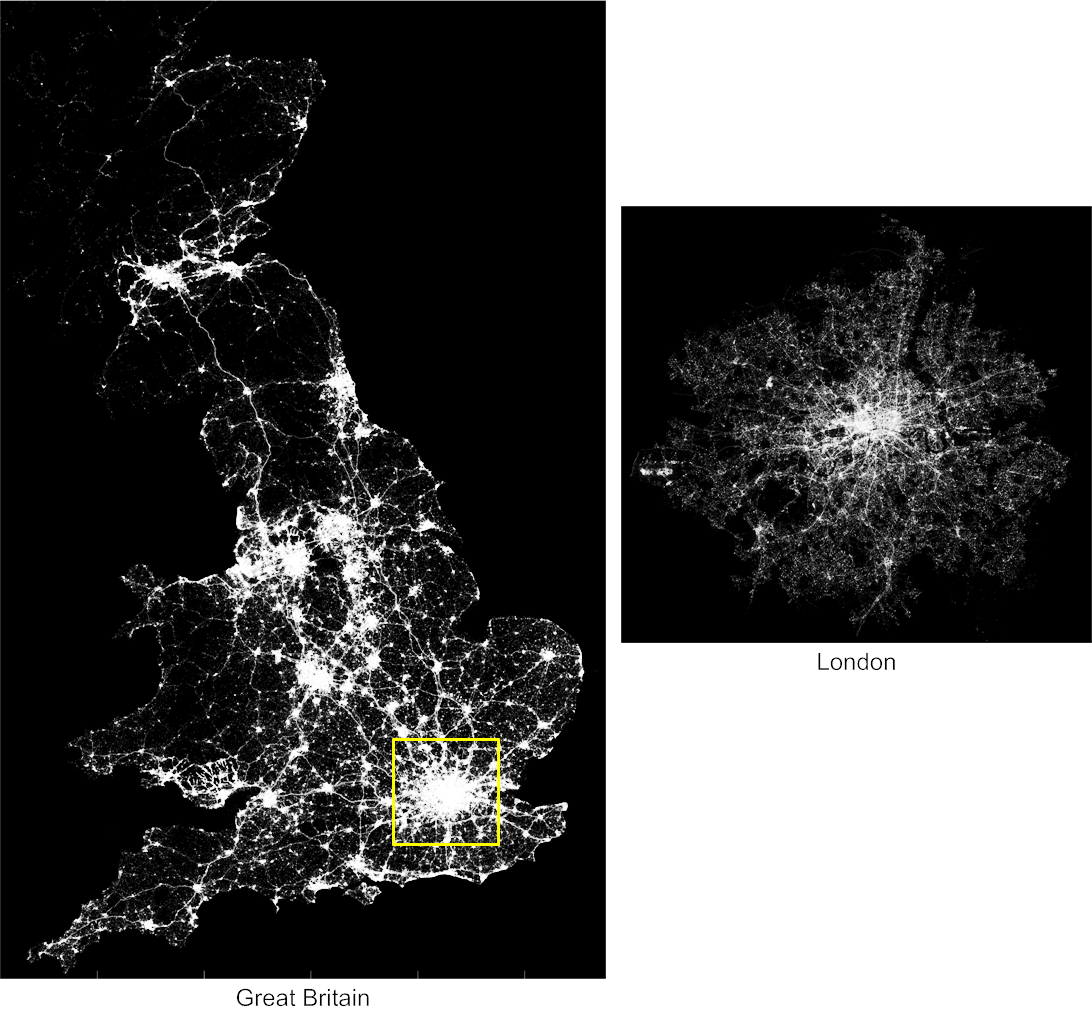
\includegraphics[width=.8\linewidth]{./figure/S2_twitter_density_Fig_1}
\caption{{\bf The spatial coverage of collected geo-located Tweets in Great Britain (left) and London (right).} Each point corresponds to an individual geo-located tweet collected for this study. Note that Twitter activities are most apparent in urban areas.}
\label{S2_Fig}
\end{center}
\end{figure}
The original location information embedded in the geo-tag is given in units of latitude and longitude.
We examined the \textit{``geo"} attribute in each raw tweet and kept the one with location information derived from GPS receiver (with high resolution) rather than from geocoding process~\citep{jurdak2015}.
We projected the points into the British National Grid (EPSG: 27700) coordinate system to reduce the complexity of the required distance calculations. 
We used the geographical boundary of Great Britain, which is derived from Office for National Statistics (ONS) of UK ({\tt{http://www.ons.gov.uk/ons}}), to further restrict the remaining tweets to be ``domestic".
Based on these restrictions, the filtered dataset contains 69,847,497 tweets made by 1,153,891 Twitter users.
To reduce the effects of tweets from non-human users, the raw tweets were further filtered using the following steps.
First we removed the duplicated messages from the dataset.
We then removed non-human users based on unusual relocation speed \citep{hawelka,jurdak2015}. 
We then examined all of the consecutive locations of each user and excluded those with relocating speeds in excess of the threshold of 240 m/s as used by \citep{jurdak2015}.
Finally, to reflect the spatial interactions of residents rather than tourists, we further impose a condition that the time interval between a user's first and last recorded tweets should be more than 30 days.
In other words, a user that is identified to have stayed in the study region more than 30 days is considered as a resident.
The filtered dataset for the following study contains 60,209,778 tweets made by 824,712 Twitter users.

At this stage, each geo-located tweet is represented as a tuple $\langle user\_id, loc, t, m \rangle$, where $user\_id$ is an anonymous Twitter user id; $loc$ is the recorded location of the tweet as a coordinate pair; $t$ is the timestamp of the tweet's post; and $m$ is the actual content of the tweet. 
We then constructed a trajectory for each Twitter user by appending all the recorded locations (with the same  $user\_id$) in the chronological order (based on the timestamps).
To protect Twitter users’ privacy, the id field was replaced with a randomly generated unique number and the content of the message was removed.
In addition, the actual location of each geo-located Tweet is only used for distance calculation and determining the corresponding geographic unit it falls in. 
Our simplified geo-located tweet dataset can be shared with other researchers upon request.

\subsection{Mobility network of Twitter user spatial interactions}
A Twitter user's movement is defined here as the individual's geographic relocation or displacement~\citep{gonzalez2008}.
This is not equivalent to a ``trip" taken by an individual, because, displacement includes situations when the time interval between two consecutive recorded locations is one month.
To identify the clusters of urban regional connectedness, Twitter user movements are used to establish a connectivity network, where two urban regions connect when a Twitter user's movement begins in one and ends in another.
These connections can be represented by an origin-destination (OD) matrix based on the collective Twitter user displacements within the dataset.
This OD matrix is essentially a mathematical representation of a weighted directed graph $G\equiv\langle V, E_{w}\rangle$, where $V$ is a set of spatial nodes corresponding to the underlying urban regions and $E_{w}$ is a set of edges representing the connections between a pair of nodes and the corresponding weights are assigned by the accumulated volume of Twitter user movements.

To build the spatial network at a national level, we had to determine the basic units to serve as spatial nodes of the connectivity network of urban regions.
Previous studies have suggested equi-distant spatial tessellation to generate nodes, which uses voronoi polygons to partition the space based on the collected points~\citep{rinzivillo2012,zhong2014}. 
This approach demonstrates improvements for estimating the locations of mobile phone records based on the cell tower triangulation~\citep{gonzalez2008,qian2013}.
However, equi-distant tessellation decreases the spatial resolution of aggregated geo-located tweets, because the location information is usually derived from the embedded GPS within mobile devices and tends to provide greater accuracy~\citep{sakaki2010}.
Another approach is to partition the space into a grid of spatial pixels~\citep{liuPopMobility,ratti2010}.
However, the size of the cell can potentially lead to biases due to the Modifiable Area Unit Problem (MAUP)~\citep{openshaw1984,wong2009}, where different choices of unit size can lead to significant variant findings. 
To compare our investigation with the findings of similar studies, and avoid subjectively deciding the cell size, we performed statistical analysis of Twitter user mobility patterns in Great Britain and measured the distribution of collective Twitter user displacements and the radius of gyrations of individuals \citep{gonzalez2008,jurdak2015}.
The radius of gyration is a metric to distinguish mobility patterns of individuals~\citep{gonzalez2008}, which is defined as Eq. \eqref{eq:1}:

\begin{equation} \label{eq:1}
r_{g} = \sqrt{\frac{1}{n}\sum_{i=1}^{n}(p_{i} -  p_{centroid})^{2}}, \textrm{where}\hspace{1ex} p_{centroid} = \frac{1}{n}\sum_{i=1}^{n}p_{i}
\end{equation}

\noindent This measures the accumulated distances of deviation from the center of mass of an individual user's trajectory, where $p_{i}$ is one of the user's locations and $p_{centroid}$ is the center of mass of the user's trajectory.
By examining the probability distributions of the radius of gyration, also known as the spatial dispersal kernel $P(r_g)$~\citep{brockmann2006}, we chose 10 km as the cell size at the national level of Great Britain (Fig.~\ref{S4_Fig} - c, with details shown in the next section). 
More importantly, as 10 km is the distinct geographic distance for separating two main groups of Twitter users in terms of the spatial coverage in Great Britain, a 10-km size cell serves as a mask to partitioning the space.
In this way, we can focus on the inter-connections among different urban regions with less attention to movements around a user's neighborhood (i.e., within 10 km radius), such as home or work places.  
Thus, we created a fishnet with 2784 10-km size cells.
The cells of the fishnet act as proxies to represent individuals' spatial coverage areas to focus more on the inter-connectivity among cells and identify strongly connected cell clusters. 

\subsection{Community structure of the network of spatial interactions}
Based on the derived mobility network of spatial interactions, which is a directed weighted graph, we further determined clusters of strongly connected spatial nodes, known as communities, in the graph space. 
There are a variety of community detection algorithms that produce different results depending the definition of community within the network~\citep{coscia2011}.
A common community detection method is based on modularity maximization~\citep{newman2006}, seen in previous studies~\citep{hawelka,ratti2010,song2012}.
However, such an approach is often problematic: it is found to have an inherent resolution problem, where small communities are either ignored~\citep{fortunato2007} or assigned with high modularity scores \citep{guimera2004}; and it is found to produce less informative partitions in many empirical networks~\citep{good2010}.
Since our graph is a directed weighted graph, the alternative community detection library documented in the literature is Infomap~\citep{domenico2015,rosvall2008}, which is considered to produce better community detection results~\citep{lancichinetti2009}.

Infomap uses the map equation~\citep{rosvall2010} to represent the probability of flow of random walks within information systems~\citep{rosvall2008}.
It identifies communities by minimizing the expected description length of the trajectory of a random walker, which is shown below:
\begin{equation} \label{eq:2}
L(M)=qH(Q) + \sum_{i=1}^{m} p_{i}H(p_{i})
\end{equation}
In Eq.\eqref{eq:2}, $L(M)$ consists of two terms: qH(Q) is the entropy of the movement among clusters and $ \sum_{i=1}^{m} p_{i}H(p_{i})$ is the entropy of movement within clusters. 
Specifically, q is the probability that a random walker jumps from one cluster to another, while $p_i$ is the probability of the in-cluster movement of cluster i.
This algorithm can be intuitively tailored to describe strongly connected clusters of urban regions based on Twitter user movement.
The detailed literatures and implementations of Infomap can be found on this website ({\tt{http://mapequation.org}}).
Note that Infomap is capable of performing multi-level community detection~\citep{domenico2015}, but we only use this algorithm to produce our most detailed community structures in order to examine groups of strongly connected urban regions.

\subsection{Distance decay effect and gravity model}
As mentioned above, the clusters of urban regions in the form of communities in the network space often yield geographically cohesive urban areas. 
This phenomenon is speculated to be related to the distance decay effects, where the interaction strength between two urban regions decreases as the geographical distance between them increases.
A gravity model is often used to express such relations, as is shown in Eq. \eqref{eq:3}, where $<T_{ij}>$ and $d_{ij}$ denote the interaction from i to j and distance between two places, $K$ is a constant, and $P_{i}$ and $P_{j}$ are the population size of place $i$ and $j$ respectively. 
The interaction strength decreasing with respect to increasing geographic distance is expressed by the distance decay function, $f(d_{ij})$, where the parameter $\beta$ reveals the distance impact on interaction strength.
A greater $\beta$ indicates stronger decay and the interaction strength is more influenced by distance~\citep{liu2014}.
While it is suggested that population size may not be an accurate indicator to describe the repulsion or attractiveness between places, the gravity model is usually fitted by using observed interaction strength and the distance between geographical entities~\citep{liu2014}.
\begin{equation} \label{eq:3}
<T_{ij}>=k*\dfrac{P_{i} * P_{j}}{f(d_{ij})},  \textrm{and}\hspace{1ex} f(d_{ij}) \sim d_{ij}^{\beta}
\end{equation}

In this study, the main purpose for adopting the gravity model is not to find the best $\beta$ value to estimate the potential interaction strength among depicted urban areas.
Interestingly, the distance decay effects are also found in human mobility patterns~\citep{zhao2016}, the authors argue that it is due to the constraints of complex urban structure.
In this study, in line with the idea that urban environments are conceptualized spaces that are recreated and formed by human activities~\citep{schliephake}, we speculate that the distance decay effects in affecting the interaction strength of two geographic regions and ultimately depicting the urban structures (e.g., urban boundaries), is contributed by (or related to) the distance decay parameters found in the underlying mobility patterns. 
In particular, since we have used a mobility network of spatial interactions, if this hypothesis stands, it will provide strong support that the depicted urban boundaries are not random artifacts but indeed reflect how naturally people move across the geographical regions. 

\section{Results}
\subsection{Collective Mobility Patterns of Twitter Users in Great Britain}
We modeled different aspects of the collective mobility patterns of Twitter users.
These patterns include: the number of visited locations per user,  the collective user displacements, and the radius of gyration of individuals in order to identify natural breaks in user travel patterns.
We then used these natural breaks within the mobility patterns to partition the geographic space of Great Britain into fine-grained cells and established the connectivity among these cells to redraw non-administrative anthropographic urban boundaries. 

We found that the cumulative distribution function of the number of locations visited by each Twitter user follows a two-tier power law distribution (Fig.~\ref{S3_Fig}). 
The majority of the data follow a truncated power-law distribution $P(X\geq x)\sim x^{-\alpha}e^{-\lambda x}$, where $\alpha = 1.24, \lambda =0.00132$; and the tail part (less than 2$\%$ of the whole population) follows a power-law distribution  $P(X \geq x)\sim x^{-\alpha}$ with $\alpha$ value is 3.2.
The distribution was found to be consistent over each month examined (June to December, 2014), which has a slight offset in the truncated power-law distribution (the mean $\alpha$ value is 1.26 $ \pm$ with a 0.05 $\sigma$ and the mean $\lambda$ value as 0.00134 $ \pm$  with a 0.0002 $\sigma$). 

The two-tier power law distribution indicates that the collective behavior of Twitter users visiting different locations can be well approximated with a (truncated) L\'{e}vy Walk (a random walk) model~\citep{rhee2011,reynolds2012}, which has also been identified in many human mobility studies using different mobility data~\citep{zhao2015}.
The similarity among the distributions suggests that the mobility data collected from geo-located tweets is temporally stable, at least at monthly intervals, which indicates that our approach using Twitter user mobility to delineate urban boundaries is viable.  
In addition, the L\'{e}vy Walk model reveals the diversity regarding the number of visited locations per user, which indicates a level of ``randomness'' in Twitter user movement across space. 
It, in turn, justifies our choice of using the map equation community detection algorithm~\citep{rosvall2008} to identify the clusters of urban regional connectedness using large-scale Twitter user movement data.

\begin{figure}[ht]
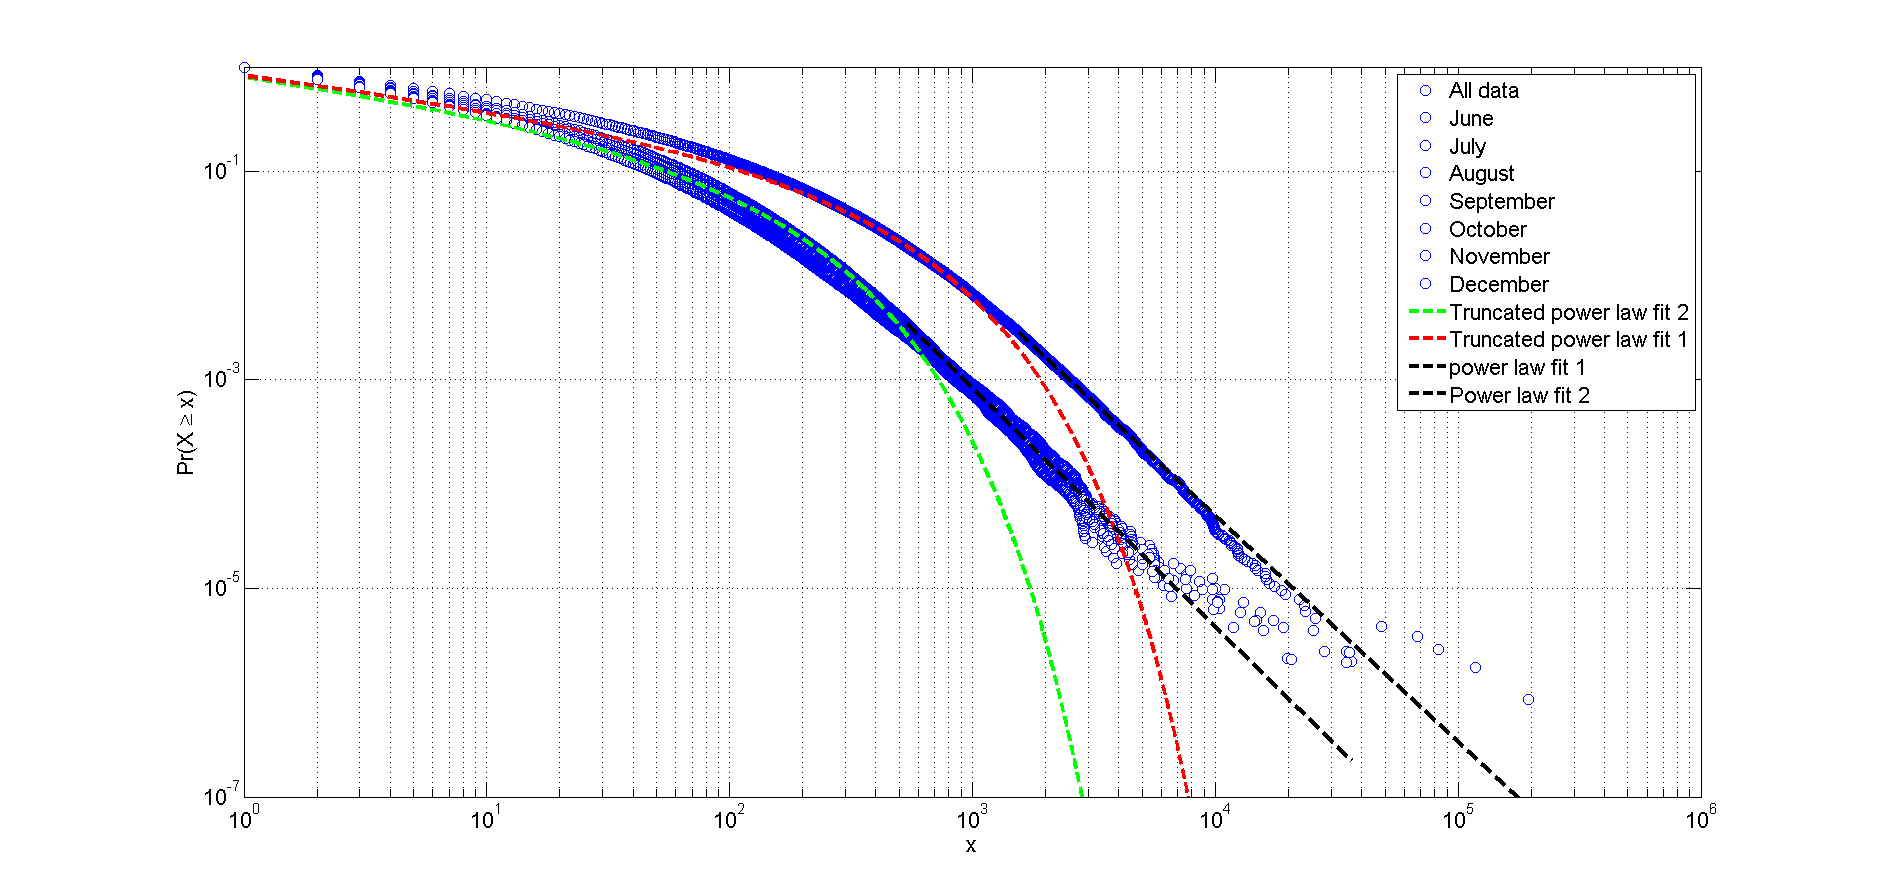
\includegraphics[width=1.0\linewidth]{./figure/S3_visitation}
\caption{ \bfseries{Cumulative distribution of the number of locations visited by each Twitter user during different timespan}}
\label{S3_Fig}
\end{figure}

We then studied two aspects of the Twitter user mobility patterns: the distribution of Twitter user displacement and the radius of gyration. 
Twitter user displacement refers to the distance between two consecutive locations in a user's trajectory using a straight-line distance metric.
The radius of gyration describes the deviation of distance from the center of mass in a user's trajectory.
The probability distributions of the collective user displacement $P(d)$ and radius of gyration $P(r_g)$ are presented in Fig.~\ref{S4_Fig}, where the fitting method for identifying different distance ranges is derived from~\citep{jurdak2015}.
The probability distribution of the collective displacements can be approximated by $P(d) \sim \lambda_{1} e^{-\lambda_{1}(d - d_{min})}, d_{min}=10m$ from [10m, 70m] (accounting for 3$\%$ of the population),  $ P(d) \sim \beta\lambda_{1}d^{\beta-1}e^{-\lambda^{1}(d^\beta-d_{min}^\beta)}, d_{min} = 100m$ from [70m, 70km] (93$\%$ of the population), and $P(d) \sim {d}^{-\alpha}$ [$>$ 70km] (4$\%$ of the population). 
The displacement distance between 70m and 100km can be further approximated by two power law distributions with a cut-off point at 4km (55$\%$ distances are less than 4km and 40$\%$ distances between 4km and 100km), which indicates the urban movement captured by the geo-located Twitter data to reveal two different modes: inter-city and intra-city movement. 
In short, these fitting functions suggest the existence of multi-scale or multi-modal urban movements captured from Twitter users in Great Britain, which means the geographically cohesive, non-overlapping urban areas identified in the next section are not just a result of short distance movement but emerge naturally from the broader Twitter user mobility pattern.
Note that a similar multiphase pattern was observed in Twitter user displacements in Australia, but with slightly different distance ranges~\citep{jurdak2015}.

Further, we analyzed the distribution of radius of gyration to understand the movement from the point of view of individual Twitter users rather than separate displacements.
The distribution of the radius of gyration of Twitter users in Great Britain can be approximated through a combination of three functions: $P(r_{g}) \sim \lambda_{2} e^{-\lambda_{2}(r_{g} - {r_{g}}_{min})}, {r_{g}}_{min}=10m$ from [10 m, 30m], $P(r_{g}) \sim \lambda_{2} e^{-\lambda_{2}(r_{g} - {r_{g}}_{min})}$ from [50m, 10km], and $P(r_{g}) \sim {r_{g}}^{-\alpha}$ [10km, 100km], where these three functions account for 92$\%$ of all the users.
This suggests that there are three primary types of users that: (1) tend to stay at one location or at nearby locations when they tweet, or (2) tend to move at the intra-city scale when they tweet, or (3)  tend to exhibit a large spatial coverage. 
(1) and (2) account for approximately 53$\%$ of all users.
Note that the accuracy of these values for defining the distance bound depends upon the accuracy of the location information of each geo-located tweet. 
These findings are consistent with the findings in the literature on human mobility, where the radius of gyration of human movement is bounded to different distance ranges~\citep{brockmann2006,gonzalez2008}.
In particular, the distribution of the radius of gyration of Twitter users over the greater London region can be fitted by similar functions.
However, as it reflects intra-city level mobility patterns, there is no distinct distance range to indicate large spatial coverage.
The distance-decay effects found in both user displacements and the radius of gyration shows evidence of spatial proximity in Twitter user movement. 
It explains that the communities of urban regions within the graph space are geographically close, but are able to be separated from other groups, which results in the delineation of urban boundaries based on the spatial interactions of Twitter users.

\begin{figure}[ht]
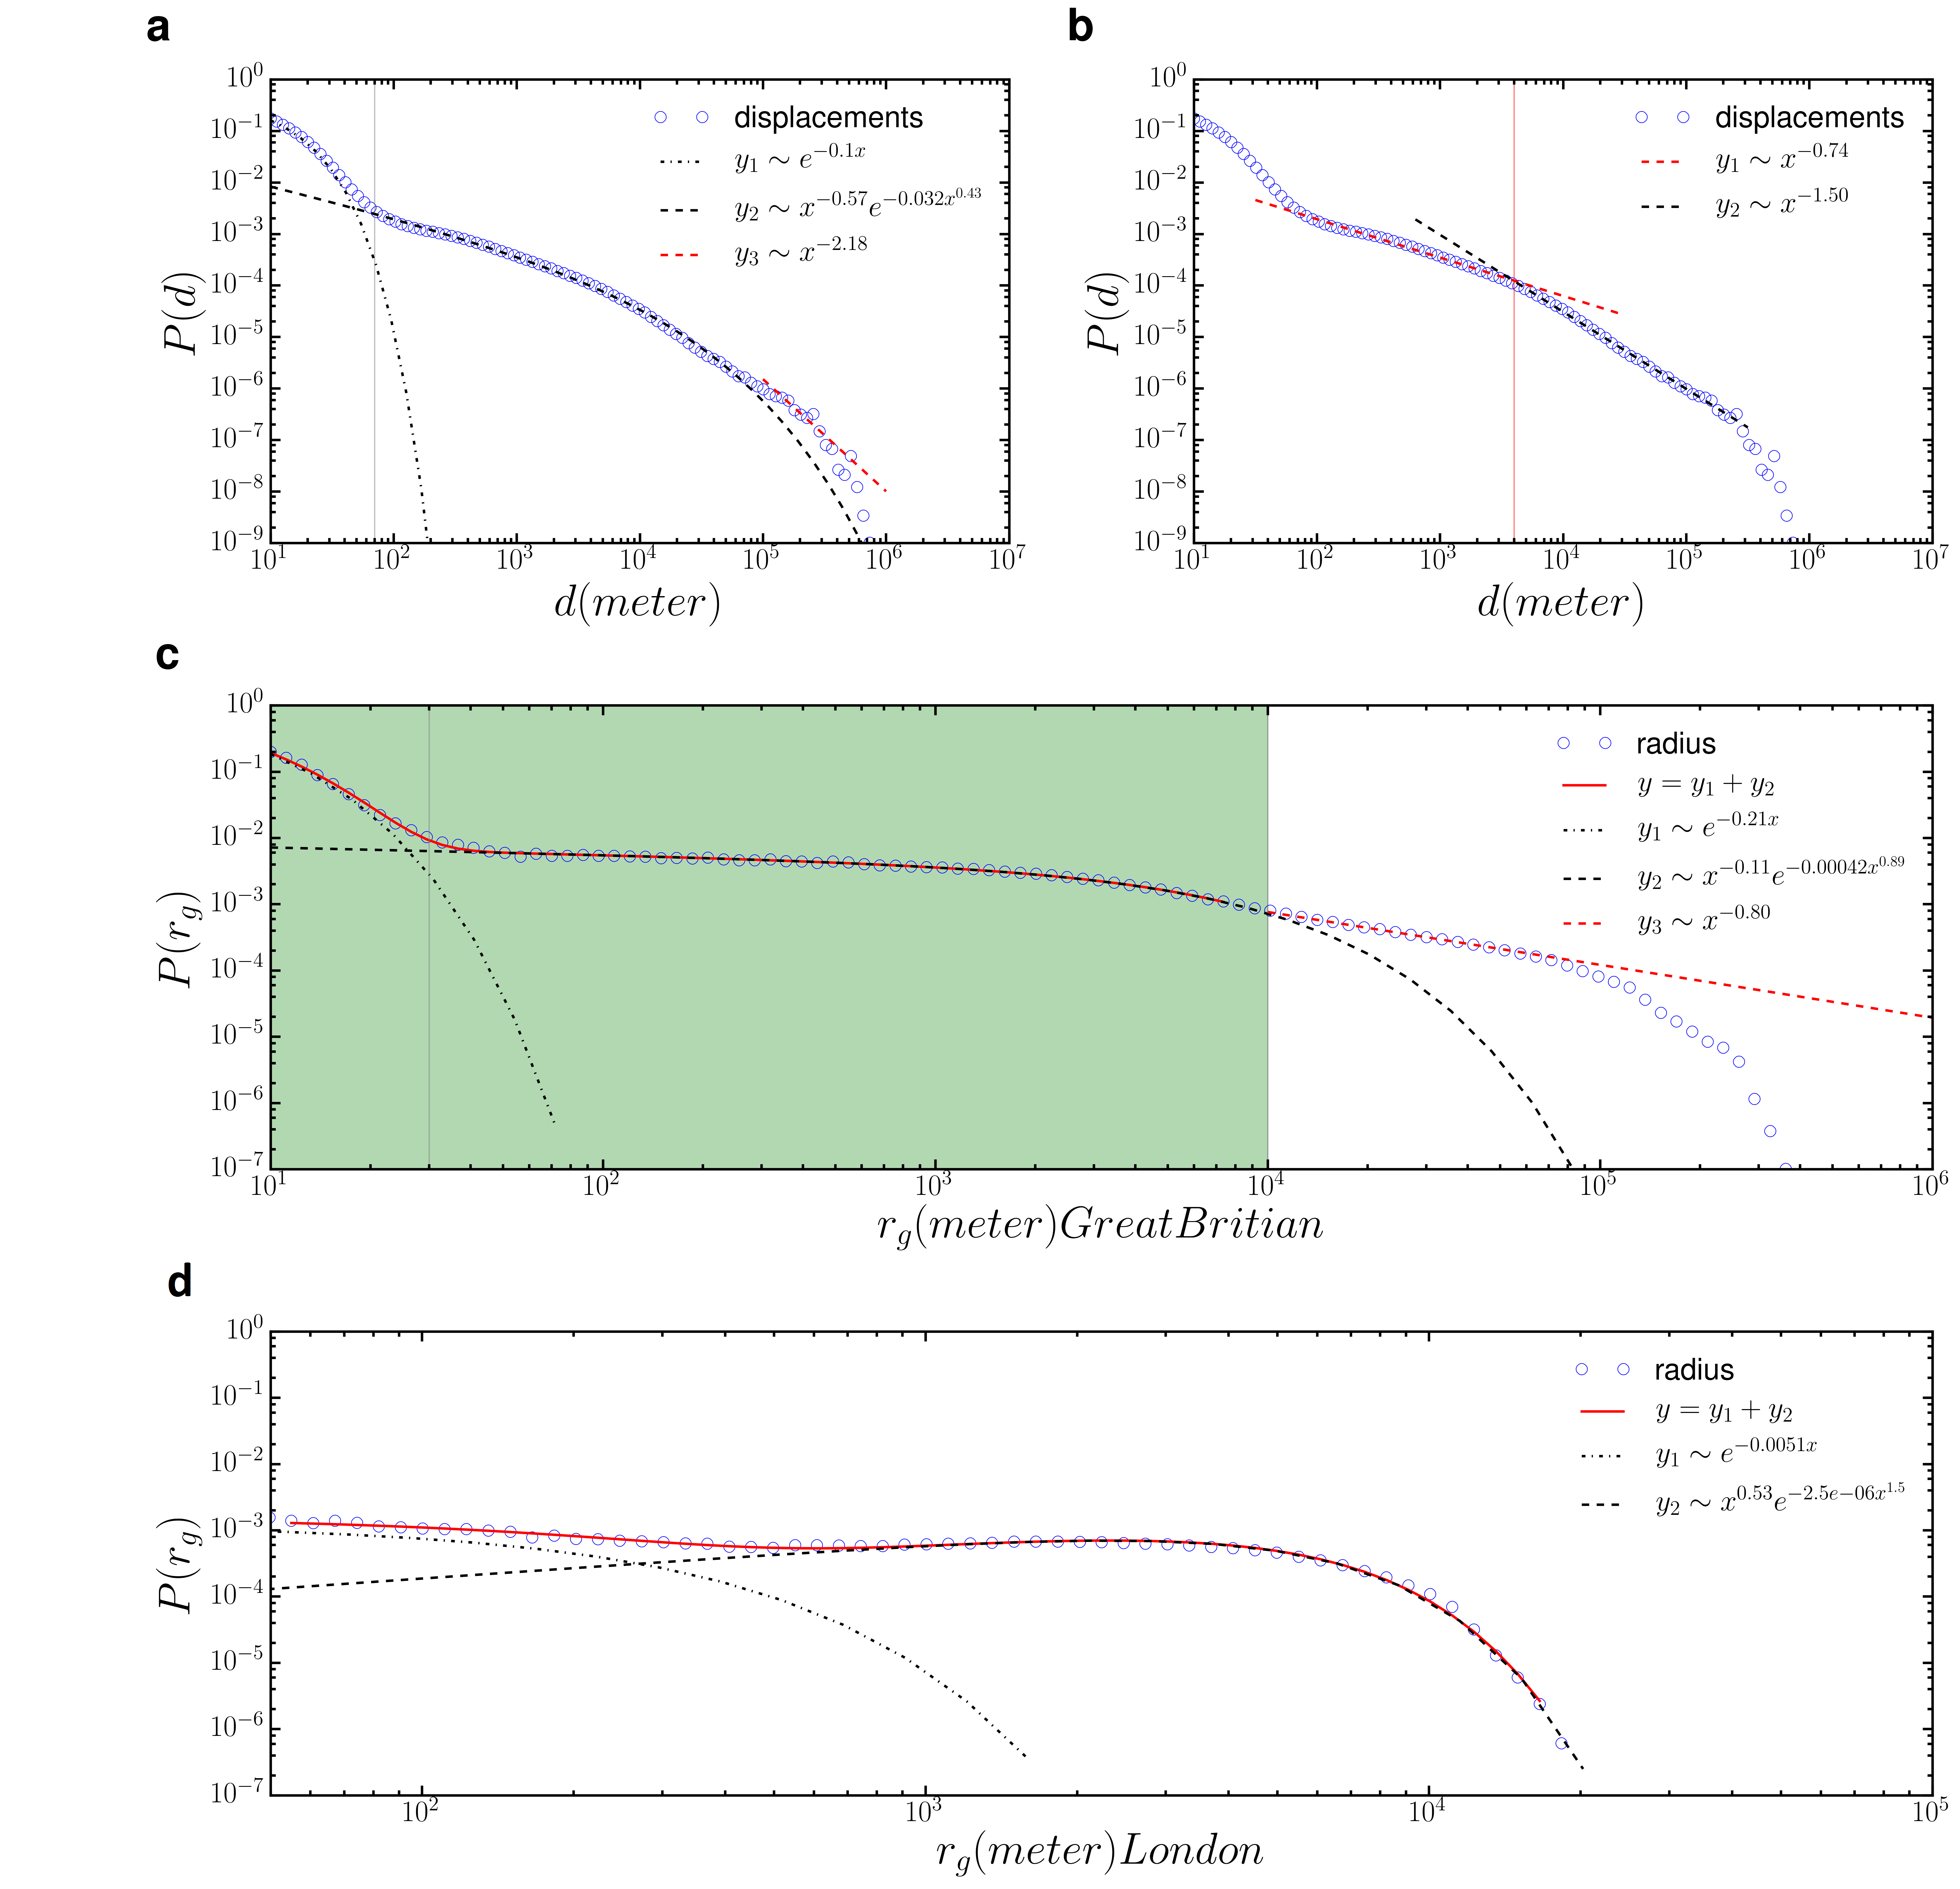
\includegraphics[width=1.0\linewidth]{./figure/S4_radius_displacement_3}
\caption{{\bf The probability distribution of Twitter user displacements and radius of gyration:} (a) $P(d)$ is approximated by an exponential, a stretched-exponential and a power-law function (b) the distance between [70m, 70km] is approximated by a double power-law functions (c) $P(r_g)$ of Great Britain is approximated by the combination of an exponential, a stretched-exponential and a power-law function. (d) $P(r_g)$ of London is approximated an exponential and a stretched-exponential function. (The green patch shows the distance range)}
\label{S4_Fig}
\end{figure}

\subsection{Redrawing Great Britain's Urban Boundaries}
The mobility network of Twitter user spatial interaction was constructed by nodes representing 10 km by 10 km fishnet cells, where 10 km is the distinct geographic distance for separating two main groups of Twitter users in terms of the spatial coverage (i.e., radius of gyration) in Great Britain (see Fig.~\ref{S4_Fig} - c).
The cells of the fishnet act as proxies to represent individuals' spatial coverage areas to focus more on the inter-connectivity among cells and identify strongly connected cell clusters.
It provides an adequate resolution for a country wide investigation~\citep{ratti2010}.
The edges of this network were derived from the number of directed Twitter user displacements between each pair of cells.
We used this connectivity network as a proxy to partition the space associated with its nodes.
Coherent geographic regions were identified as individual fishnet cells showing more internal user movement compared to user movements across the cell boundaries to neighboring cells.
To help readers that are not familiar with the geographic context in Great Britain better interpret the derived boundaries,
we had added two additonal layers (i.e., locations of airport fields and population-wighted-centroids of workplace zones in the Great Britian) in the background of the figures.
Fig.~\ref{S5_Fig}  presents the delineated urban boundaries based on Twitter user displacement distance less than 4 km, greater than 4km, greater than 10 km, and using all available displacements together compared to the administrative boundaries of Great Britain.
One clear observation in both the coarse and fine delineations is that most of the geographic divisions are centered around big urban cores with relatively high populations.
These results are expected given that most of the tweets originate in urban centers.
However, what is remarkable is the performance of this approach in dividing the remaining space between cities.
We found that restricting the trip distance results in different delineations of the catchment area around these centers.
For example, one could explain these effects as a manifestation of the underlying gravity law~\citep{simini2012} and the distance decay effect on attracting movers~\citep{gonzalez2008}.
Remarkably, our approach performed well in terms of dividing the entire space with minimum gaps.
Empty cells were found in regions where no, or few, Twitter users had visited (e.g. forests, agriculture) especially when restricting the analysis to short distance Twitter user displacements.

\begin{figure}[ht]
\begin{center}
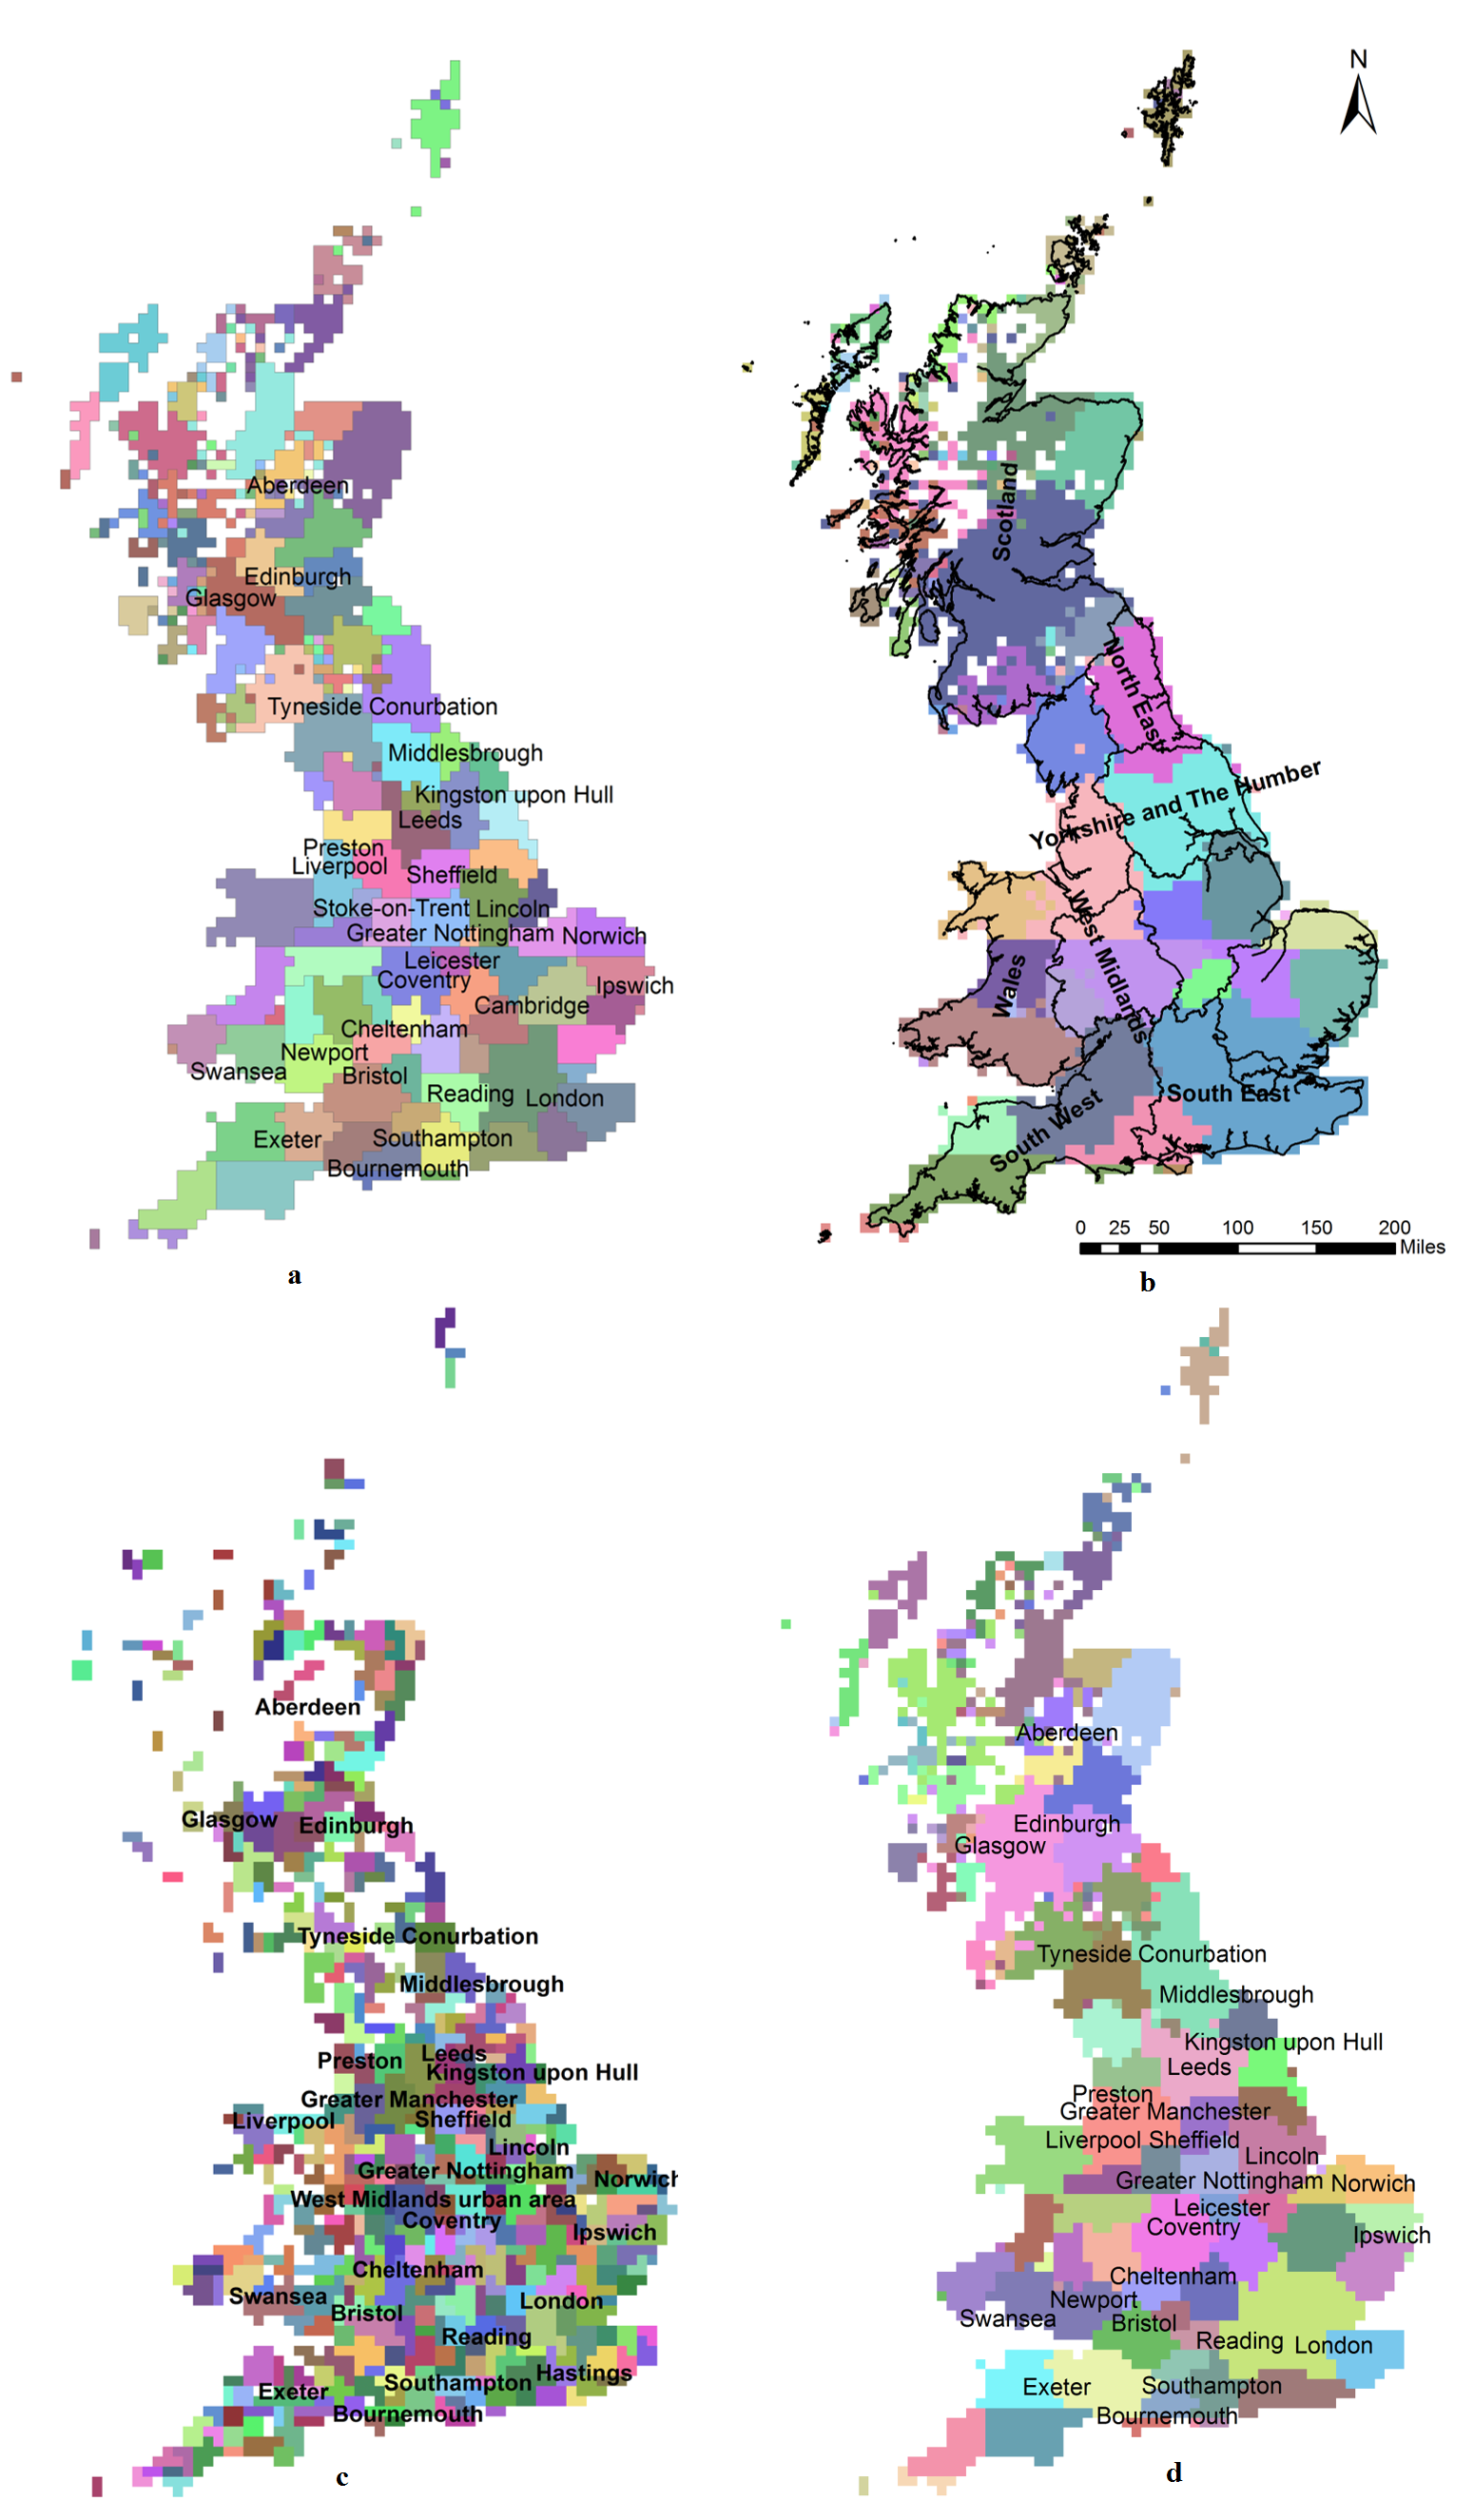
\includegraphics[width=0.9\linewidth]{./figure/S5_community}
\caption{{\bf The community structure from collective Twitter user displacements reveals non-administrative anthropographic urban boundaries} (a) all displacements with $L(M)= 7.8$. (b) displacements longer than 10 km ($L(M)=8.5$), red symbols are the locations of airport fields in the Great Britain (c) displacements shorter than 4 km ($L(M)=4.5$) (d) and displacements longer than 4 km ($L(M)=8.1$).The partition of space was done using a 10 km fishnet for the directed displacements from and to each cell. Each color represents a unique community with more Twitter users displacements among the cells compared to others. Major cities (urban audit functional areas) and NUTS are displayed as labels.}
\label{S5_Fig}
\end{center}
\end{figure}

Regional boundaries inferred from short distance Twitter user displacements (less than 4 km) exhibit very small and fragmented regions, which is probably related to daily commuting around a user's home location. 
Redrawing the boundaries based on longer distance displacements produces more cohesive, large regions.
For example, by partitioning the space based on displacements greater than 10 km created regions that are comparable to the NUTS (Nomenclature of Territorial Units for Statistics - 1) regions (Fig.~\ref{S6_Fig} - a). 
However, the power of this novel mapping technique is not to reproduce the partitions already known, rather it is to point out some of the unexpected boundaries.
For example the boundaries between England and Wales were found to be more diffuse compared to the abrupt boundary of England and Scotland.
Moreover, the city of London has a wider visitor catchment area that extends beyond the authoritative boundaries of the city.
Increasing the displacement distance results in revealing the large region connected to London (Fig.~\ref{S6_Fig}). 

Using Twitter user mobility to delineate non-administrative anthropographic boundaries enables the researcher to redraw the city at different mobility ranges inferred objectively from the user's collective distribution. 
In addition, the distance range of the movements is usually explained by local socio-economic factors (e.g., work commuting ) that provide for a specific interpretation of the apparent patterns.
The patterns obtained from Twitter user mobility are comparable to the patterns produced by those of the network of landline phone calls~\citep{ratti2010}.
For example, the region of Wales appears to consist of three communities as found in the connectivity of both phone calls and long distance movements. 
However, the regions extracted from the mobility network seems to be more spatially consistent with minimal spatial gaps compared to the partitions extracted from land-line call networks in Great Britain~\citep{ratti2010}.

\begin{figure}[ht]
\begin{center}
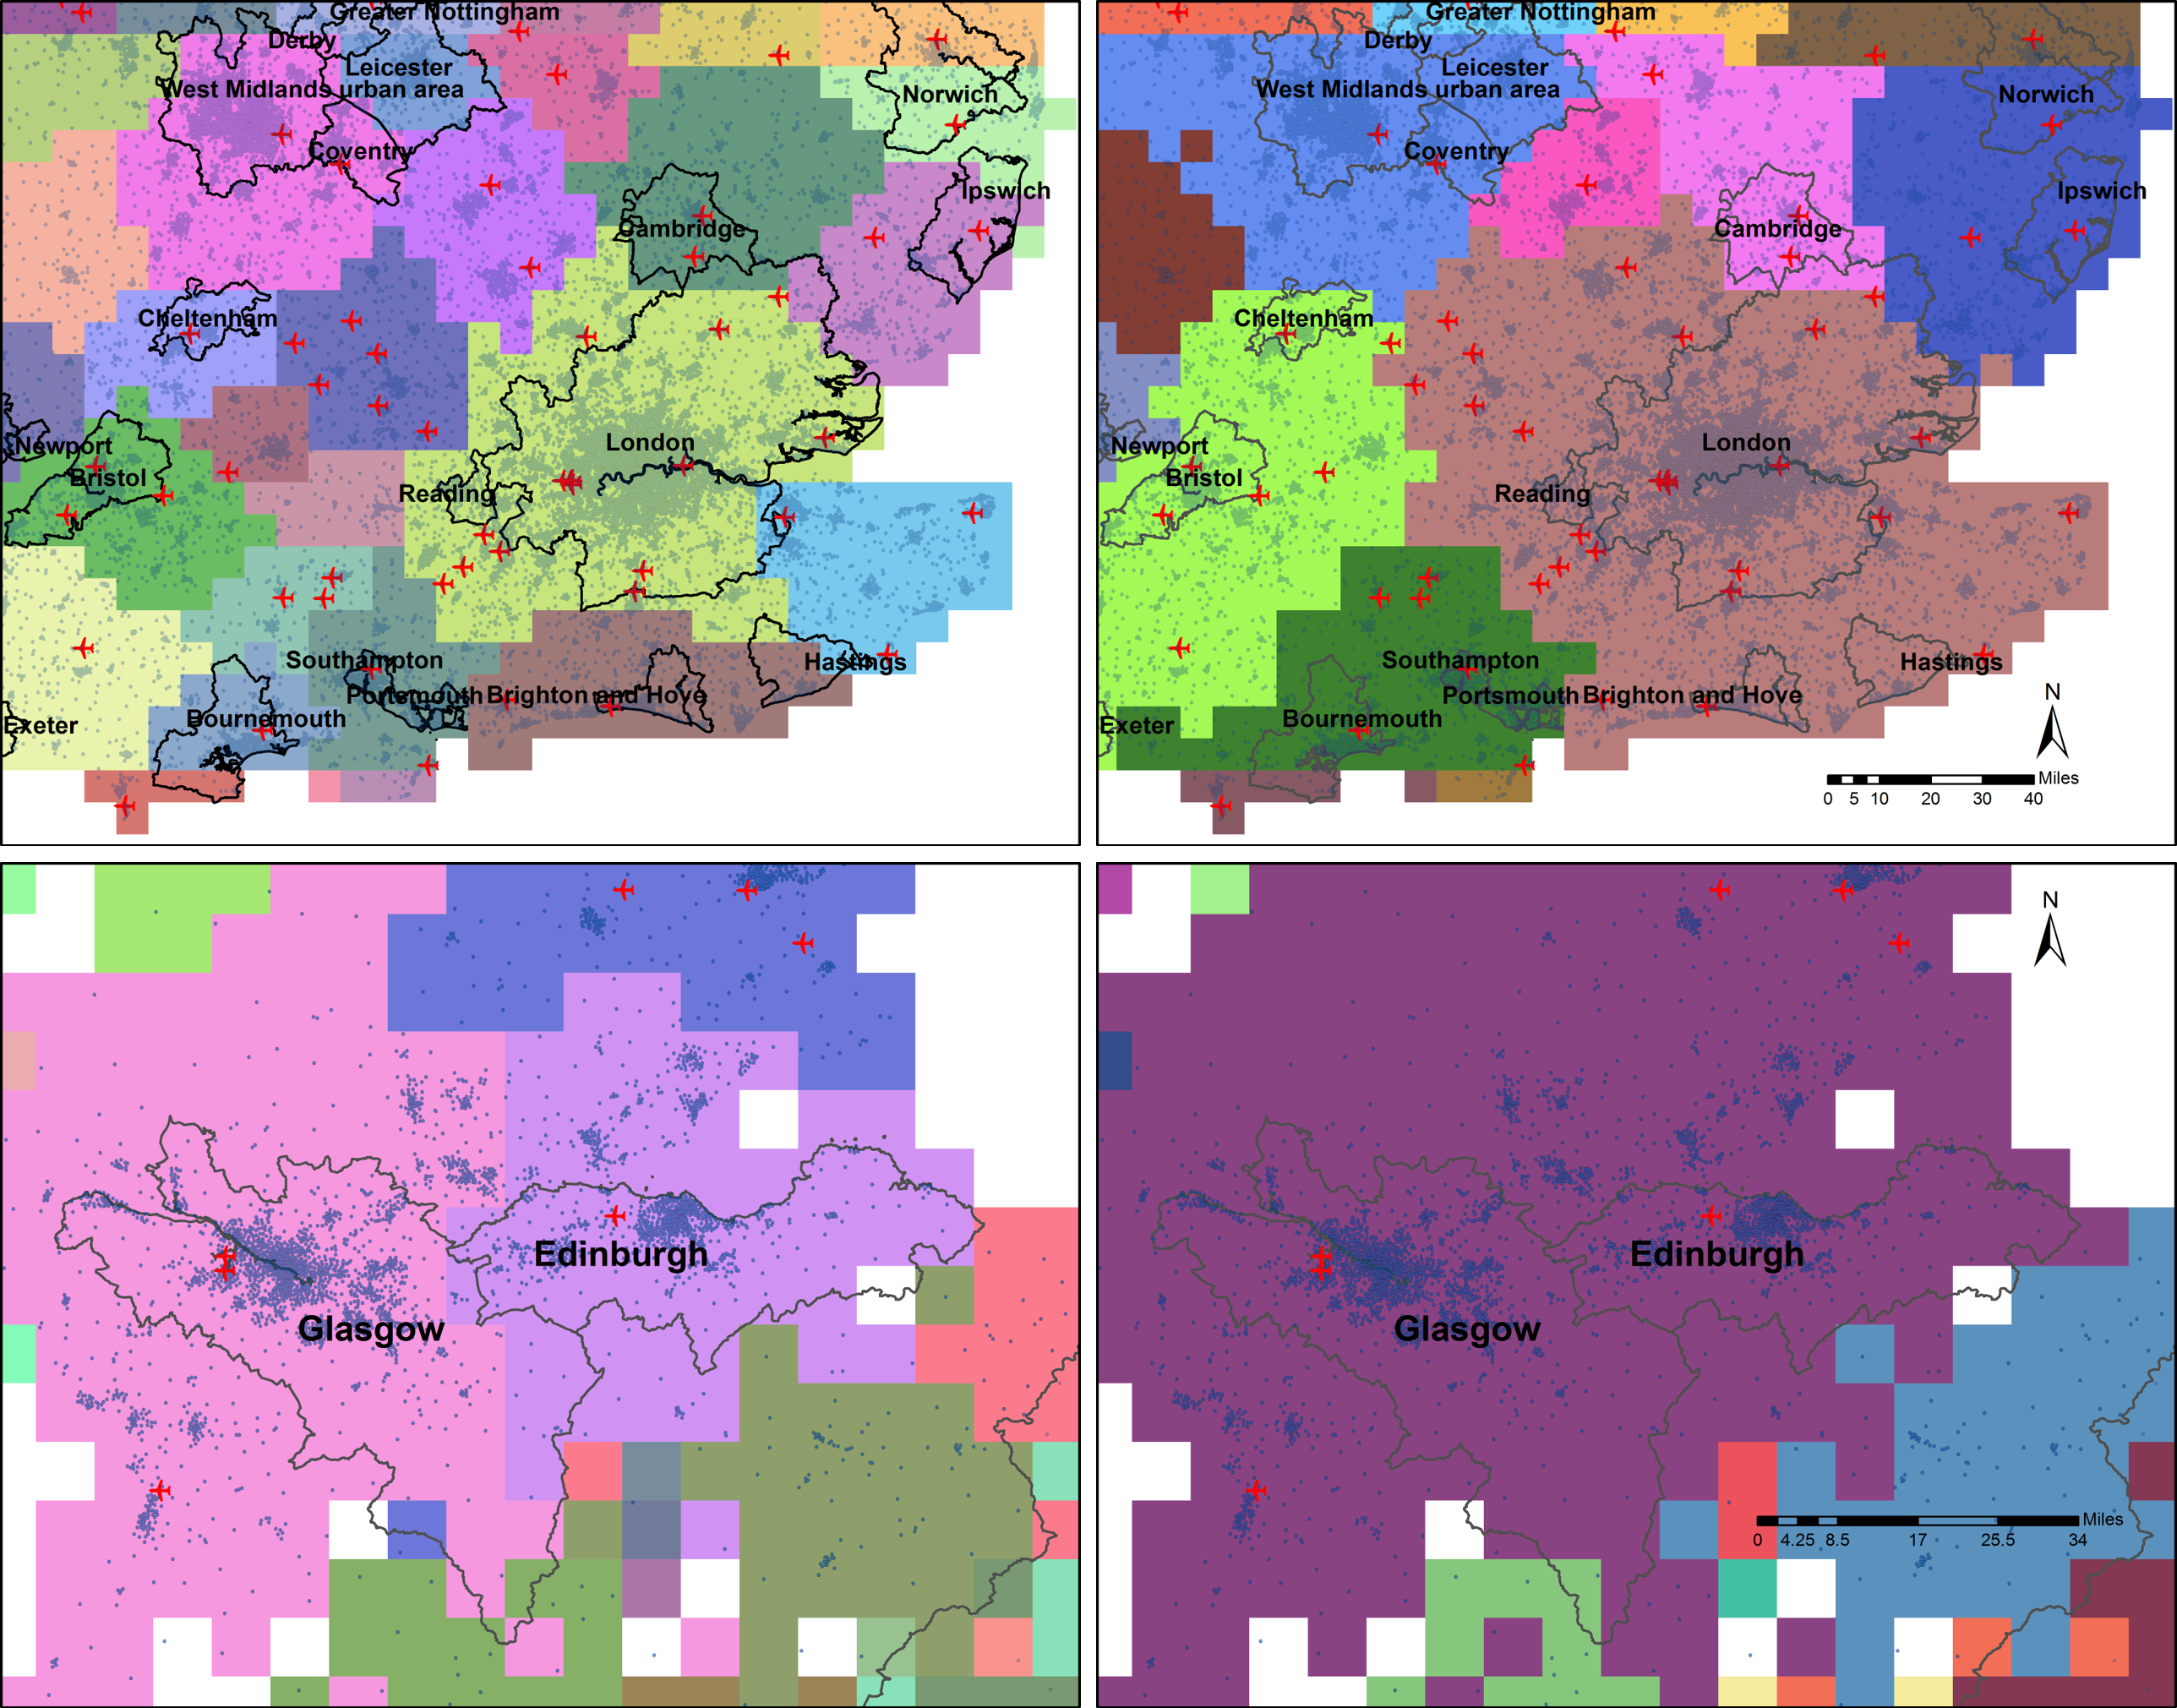
\includegraphics[width=1.0\linewidth]{./figure/S6_community_london}
\caption{{\bf The non-administrative anthropographic regions inferred from Twitter user displacements greater than 4 km (left) and 10 km (right) in comparison with major cities in England (upper figures) and Scotland (bottom figures).}  Each color represents a unique community. Including short distance movements has increased the power to differentiate the influence of nearby cities such as Glasgow and Edinburgh (lower left), while restricting the analysis to longer distance movements grouped travelers from the two previous cities into the same community (lower right). Red symbols are the locations of airport fields and gray points are the population-wighted-centroids of workplace zones in the Great Britian.}
\label{S6_Fig}
\end{center}
\end{figure}

A more detailed study was conducted over the greater London region revealing the intra-city spatial interaction patterns.
Since the captured Twitter user movements were on intra-city level (in comparison to the national level in Fig.~\ref{S4_Fig}-c), there was no distinct distance range to separate Twitter user spatial coverage in terms of radius of gyration (see Fig.~\ref{S4_Fig}-d). 
We chose 1-km cell size as referred from the related literature~\citep{liu2015}, which suggested 1-km cell size is detailed enough to depict urban structures.
The spatial partitions derived from a fine grid of 1km used all available Twitter user trips without any restriction on trip distances yields geographic boundaries comparable to some of London's boroughs  (Fig.~\ref{S7_Fig}).
However, some areas are shown to be more cohesive and display greater spatial interactions across the administrative boundaries, for instance, central London.
Although, these results suggest that travelers seem to be localized over certain areas of the city most of the time, some regions do exhibit long distance interaction patterns.
For example, the separate geographic areas in the south of Hillingdon which includes Heathrow Airport exhibits more connectivity to central London than its surrounding areas, which is explained by the usual flight passenger routes.
The technique also reveals some of the emerging communities around the borders due to the spatial intermingling of both communities.
For example, East Barnet and West Enfield seem to have higher interactions than those resulted from in the emerging cohesive zone between the two boroughs.

\begin{figure}[ht]
\begin{center}
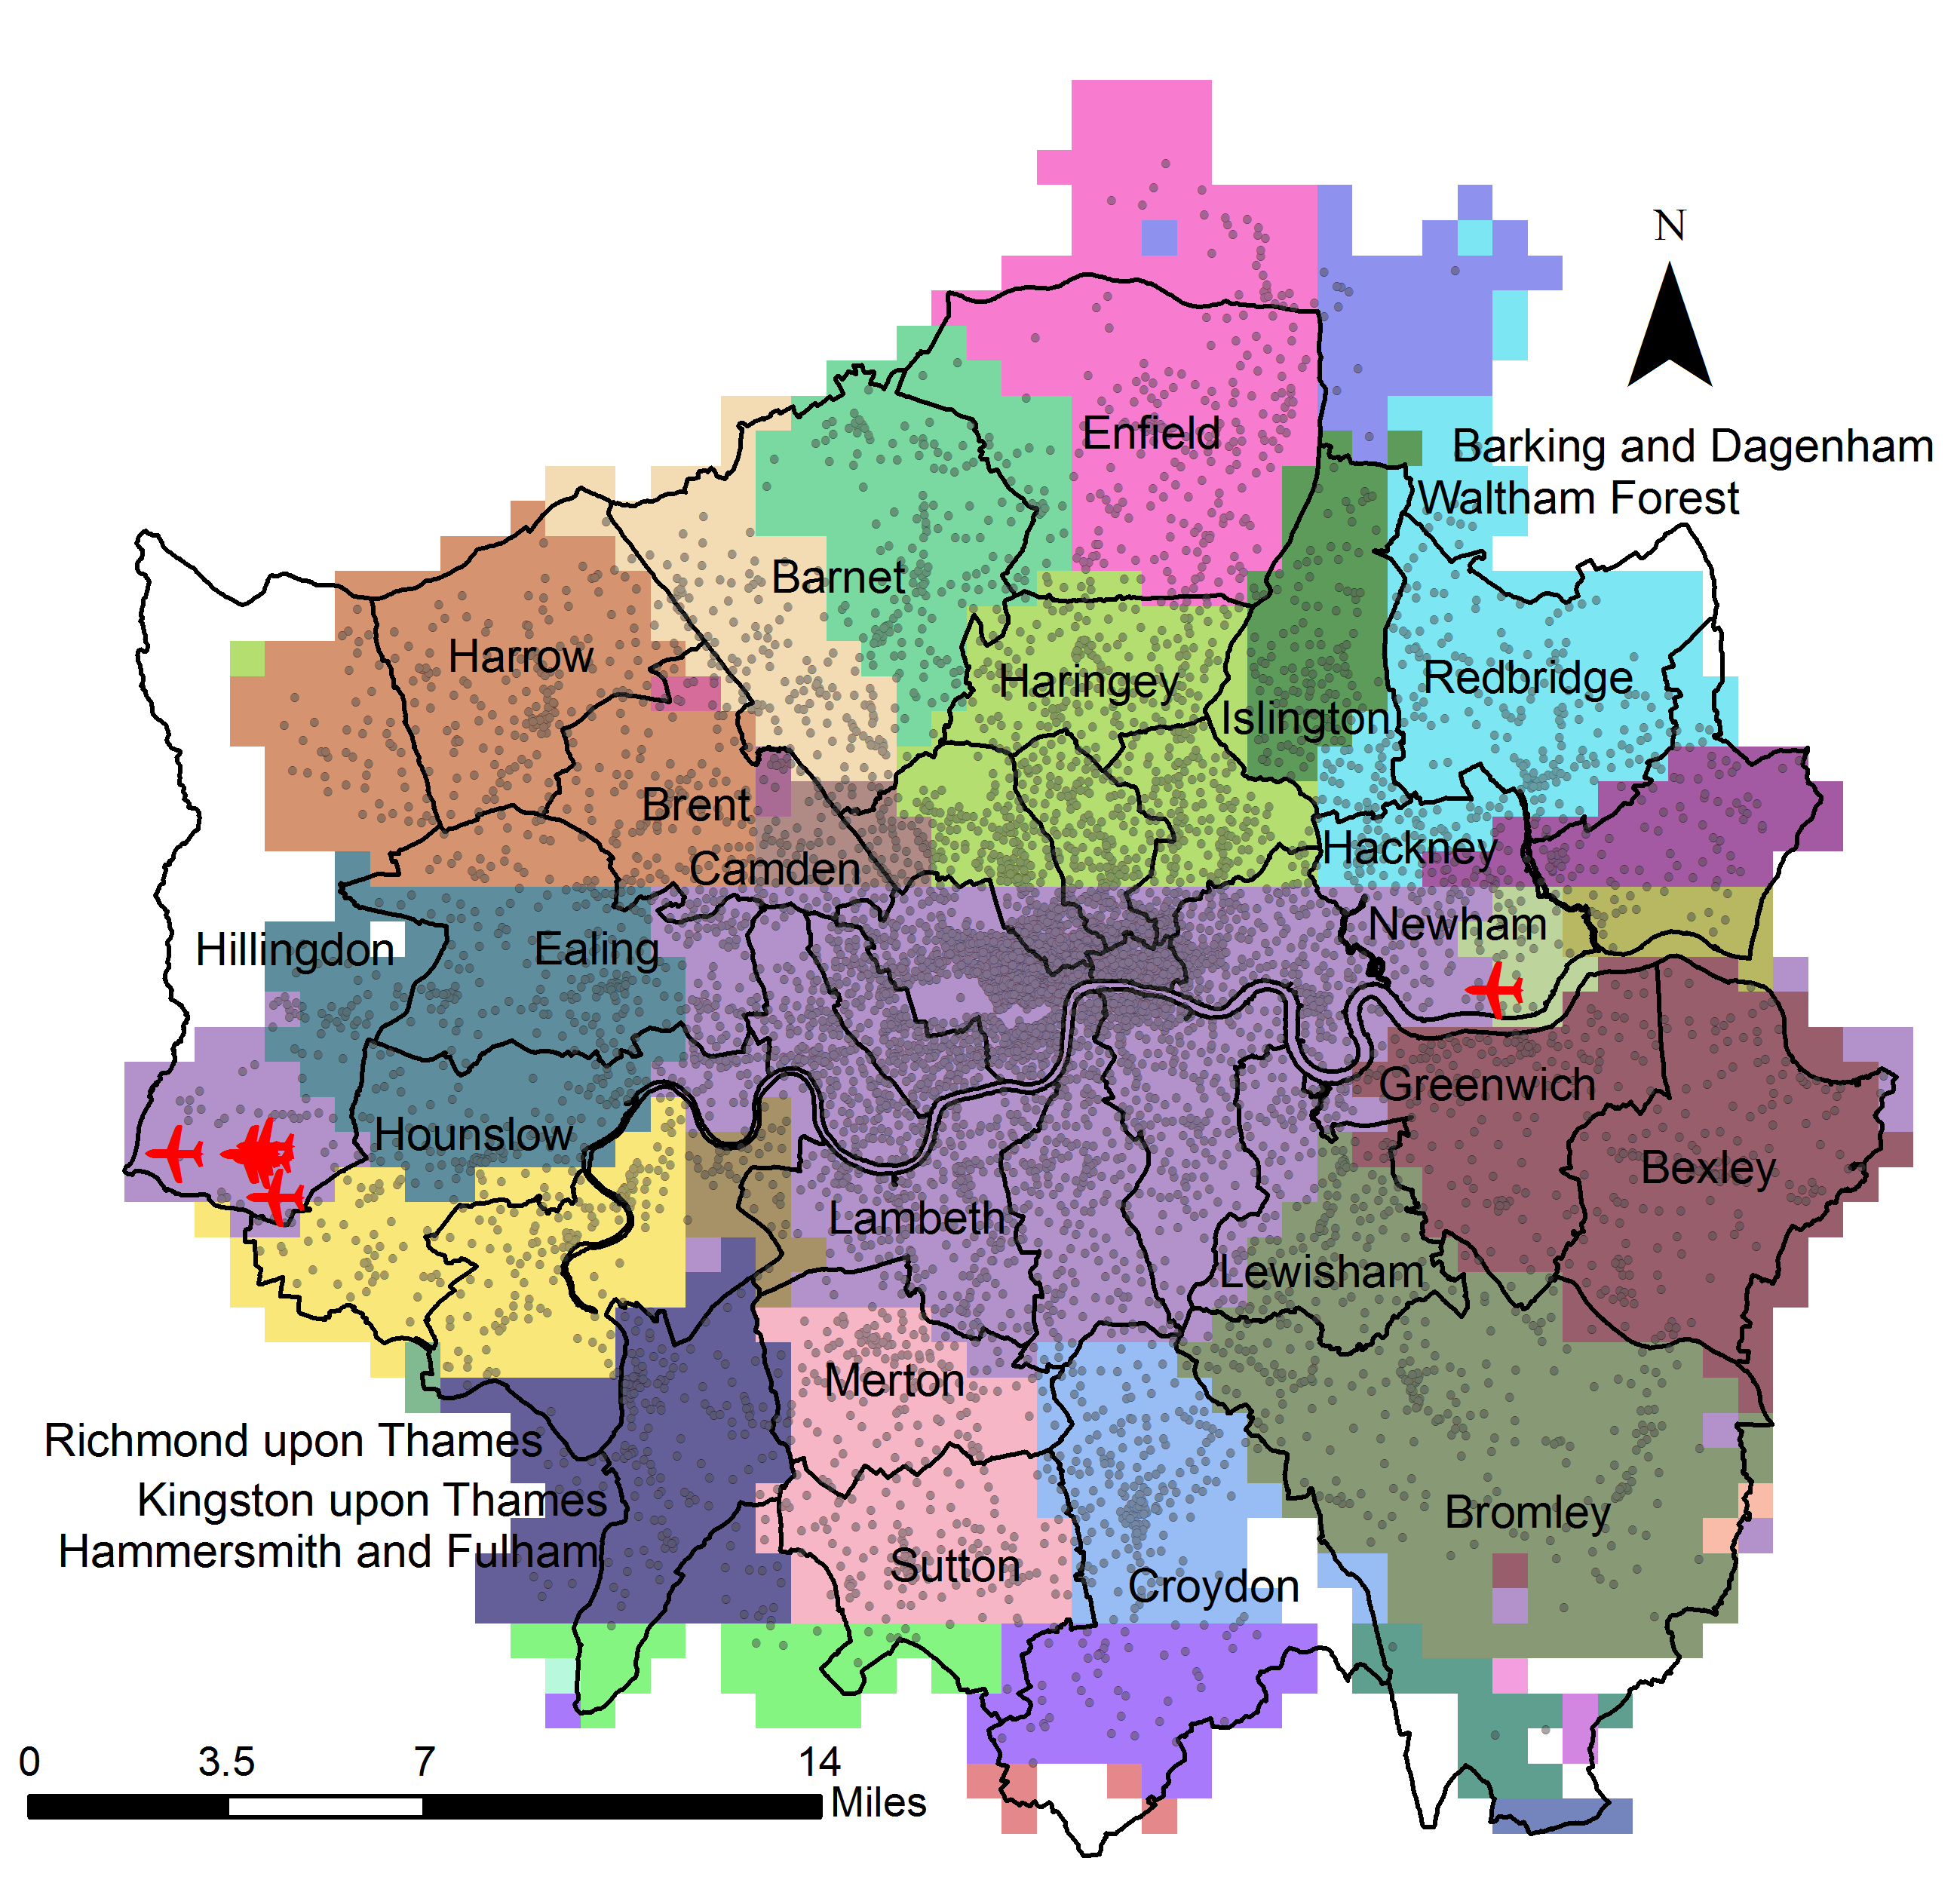
\includegraphics[width=0.9\linewidth]{./figure/S7_london}
\caption{{\bf Non-administrative anthropographic boundaries inferred from collective Twitter user displacements in the city of London compared to the boundaries of London boroughs ($L(M)=8.1$)}  A fine fishnet of 1 km cells were used to identify the detailed connectivity patterns based on all the Twitter user displacements in the area.  Each unique color represents a different non-administrative anthropographic region. Notice that some remote regions like the airport (light purple region in south of Hillingdon) share the same class with downtown because it is well connected despite the geographic separation. Red symbols are the locations of airport fields and gray points are the population-wighted-centroids of workplace zones in London.}
\label{S7_Fig}
\end{center}
\end{figure}

\subsection{Explaining the distance decay effect with a gravity model}
The results of strongly connected urban regions in the form of communities, which are derived from the mobility network of Twitter user spatial interactions, yield geographically cohesive, non-overlapping urban areas. 
While it provides a clear delineation of the non-administrative anthropographic urban boundaries of Great Britain, the reasons on why they are geographically cohesive and non-overlapping or why the boundaries stop/emerge at certain spatial extent that leads to different size of the urban areas are not clear. 
As the depicted urban boundaries exhibit a strong instance of spatial proximity, a gravity model is employed (Eq. \eqref{eq:3}) to explain how distance decay effects found in the mobility patterns affect the interaction strength between the derived non-administrative anthropographic urban areas.

In this model, the distance between two derived urban areas is measured by the geodetic distance between the centroid locations of the two.
As it is mentioned above,  $P_{i}$ and $P_{j}$  are the observed interaction between urban area $i$ and $j$, which are measured by the aggregation of movement flows in each urban area.
In particular, we set the distance decay parameter $\beta$ value as 0.8: (1) As we hypothesize that the distance decay parameters found in the underlying mobility patterns potentially contribute to $\beta$ in the gravity model (2) and we chose the 10 km cell-size based on the collective Twitter user mobility pattern regarding radius of gyration, where the distance decay parameter is 0.8 when radius of gyration $r_{g} > 10 km$ (Fig.~\ref{S4_Fig}(c)).
We found that the gravity model indicates strong linear correlation between the observed versus the estimated interaction strength with $R^{2}$ = 0.89 and $p-value < 0.01$.
This confirms that the depicted urban areas are instances of spatial proximity effects, where the strength of human (in this case, Twitter user) spatial interaction between two urban regions decreases as the geographic distance between them increases. 
The well fitted gravity model provides support that the depicted urban areas are not just random artifacts but reflect how naturally move across geographic regions.
More importantly, since we have used a mobility network to delineate the boundaries, the distance decay effects are well related and explained by the distance decay parameters found in the underlying mobility patterns.
To elaborate, the spatial interaction strength decreases along with the decay for the probability of longer distance Twitter user movements, and eventually stops at certain spatial extent, which leads to more geographically cohesive cluster of urban regions.


\begin{figure}[ht]
\begin{center}
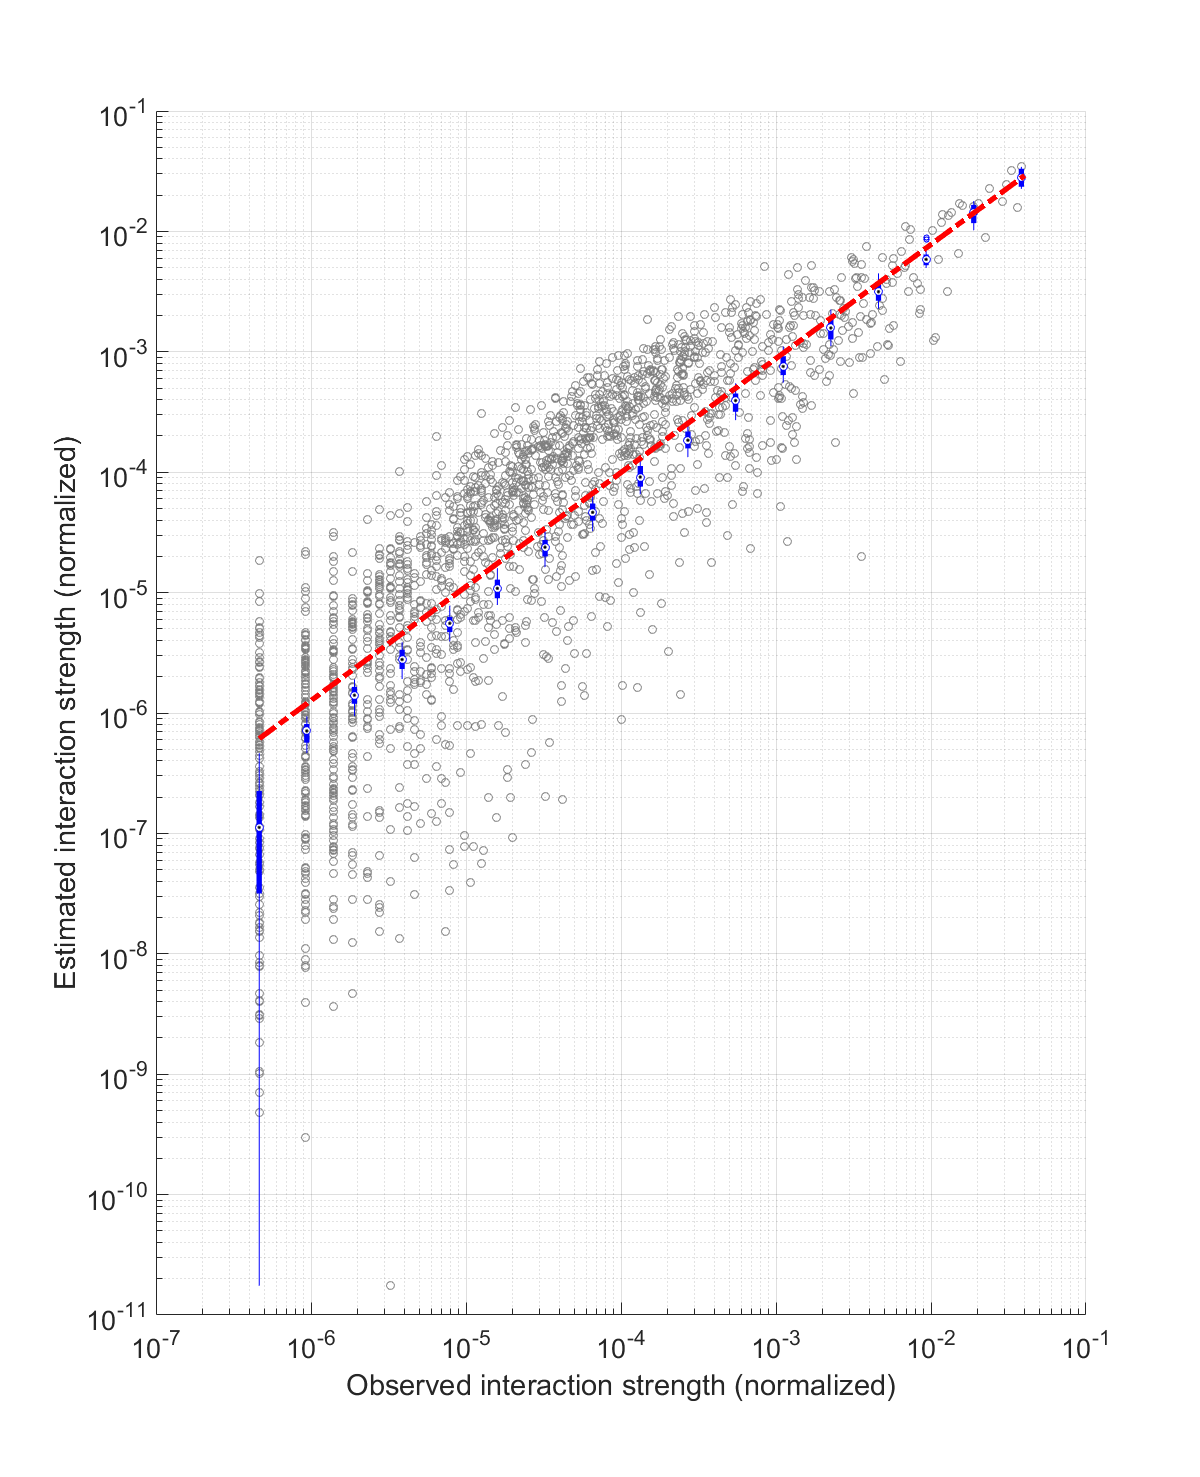
\includegraphics[width=0.7\linewidth]{./figure/Gravity}
\caption{{\bf The observed interaction strength versus the estimated ones from the adopted gravity model with $\bf{\beta}$ = 0.8 } Note that the $\beta$ value is taken from the probability density function of radius of gyration when $r_{g} > 10 km$. The red dash line indicate strong linear correlation between the estimated and observed interaction strength with $R^{2}$ = 0.89 and $p-value < 0.01$.}
\label{S8_Fig}
\end{center}
\end{figure}

%\clearpage
\section{Discussion}
It is worth noting that constructing a mobility network of spatial interaction using geo-located Twitter data has some potential concerns to limit the results from this study.
First, the geo-located Twitter data is not able to generalize to the entire population.
As the demographic information of the Twitter users cannot be easily identified, the results of delineated urban boundaries may not reflect a complete real-world image from human movements. 
The demographics of Twitter users in this study can be an under/over-representation of the all overall population in Great Britain.
Related studies have been carried out to examine the demographic information in geo-located Twitter data~\citep{steiger2015,luo2016,huang2016}, which should be carefully considered in future studies.
Second, regarding the concern of spatial sparseness of geo-located Twitter data~\citep{steiger2015}, the urban regions that do not have any, or limited, Twitter coverage can be missed during the delineation process.
To investigate whether this limited the ability to capture the connections made through Twitter user movements between urban regions, we visualized the flows of Twitter user movements using the method mentioned in~\citep{rae2009}(see Supplement Materials section 1). 
The outcome showed that the Twitter user movements in this study connected most urban areas in Great Britain and clearly exhibited long and short distance movements, where was essential for investigating the connection strength between urban regions.   
Third, since the collective radius of gyration was used to determine the cell-size in the network, we examined the temporal stability for the measurement in the geo-located Twitter data.
The probability distributions of the radius of gyration for Twitter users in the Great Britain are verified to be consistent across different monthly time span (see Supplement Materials section 2), which indicates the stability of using such measurements in this study.  
Finally, as the geo-located Twitter data offers easy data accessibility, our methods can be reproduced for other countries. 
Along with the large sample size and spatial coverage, geo-located Twitter data demonstrated its applicability for this study.

A major component in this study was imposing a virtual fishnet to partition the geographic space over Great Britain.
Alternatively, we had used the ward divisions as spatial units for aggregating Twitter user movements, which is the finest administrative boundaries of Great Britain (see Supplement Materials section 3).
Without looking into the details of the results, the derived communities in the network space are similar to the ones from using fishnet approach.
The strongly connected communities also yield geographically cohesive, non-overlapping urban areas.
However, as the ward division is still defined by administrative purpose, the polygonal units tend to be geographically continuous.
It causes problems to aggregate regions that do not have Twitter coverage into certain clusters.
Aggregating Twitter user movements at the ward level also imposes more apparent concerns of the mismatch of the overall population, where less populated areas were overly represented and connected into large areas.
These are the reasons why we chose a virtual fishnet approach for this study.

We should be aware that using different fishnet cell-size to partition the space will produce different mobility networks, and can potentially lead to different delineations of the urban boundaries.
As it is discussed above, we chose 10 km as the cell-size of the fishnet at national level in this study.
We also carried out an experiment by arbitrarily setting the cell-size to 5 km at the national level (see Supplement Materials section 4).
Note that the cell-size could be set to any value, such as 4.9 km or 5.1 km.
The fishnet with smaller cell-size (i.e., 5 km) produced more and smaller strongly-connected communities within the network space.
It indicates that the spatial resolution of the fishnet cells does affect the outcome from the community detection method employed in this study, where fishnet with smaller cell-size leads to more discrete and locally connected (i.e., smaller) clusters of urban areas.
Such an effect can be explained by the probability distributions of the radius of gyrations of individual Twitter users.
The probability of distance that deviates from a user's center location decays with a stretched-exponential function from [50m, 10km], which means the movements from Twitter users with smaller spatial coverage dominate the delineation of the connected urban areas.
To avoid arbitrarily deciding the cell-size, we studied the probability distributions of the radius of gyrations of individual Twitter users and selected 10-km as the cell-size, which is the distinct geographic distance for separating two main groups of Twitter users in terms of their spatial coverage at the national level.
In addition, this choice enabled us to focus on the inter-connections among different urban regions with less attention to movements around a user's neighborhood (i.e., within 10 km radius), such as home or work places.

To apply the map equation algorithm, the mobility network should be organized as a weighted and directed graph, on which we confirmed an undirected graph cannot lead to a meaningful result (see Supplement Materials section 4).
Since we used different physical movement ranges of users in delineating the urban boundaries, the description length $L(M)$ appeared to get larger when longer displacements were used, which corresponded to less and larger geographically cohesive, non-overlapping urban areas.
We believed that different movement ranges of users changed the weights of this graph and affected the interaction strength between two fishnet cells.
As we have illustrated that the geographically cohesive, non-overlapping urban areas were instances of spatial proximity effects, where the employed gravity model model suggested the interaction strength between two fishnet cells decreases as the geographical distance increases, the longer displacements were used, the larger $L(M)$ were produced from the map equation algorithm.

\section{Conclusion}
In this study, we presented a method that connected human mobility research with the delineation of the non-administrative anthropographic urban boundaries in Great Britain using a mobility network of Twitter user spatial interactions.
In contrast to administrative urban boundaries, our ``bottom-up" approach imposed a virtual fishnet over the islands of Great Britain to partition the space.
By studying the probability distributions of the radius of gyrations of individual Twitters users, we selected a cell-size of 10 km at the national level and 1 km for the greater London region.
Twitter user movements were used to establish a connectivity network of the fishnet cells.
Then we applied the map equation algorithm to partition the network and associated geographic regions.
The strongly connected communities within the network space yields geographically cohesive, non-overlapping urban areas that provides a clear delineation of the urban boundaries in Great Britain.
By performing a statistical analysis of Twitter user mobility patterns in Great Britain, in particular the distribution of collective Twitter user displacements, we found multi-scale and multi-modal urban movements that were divided into several distance ranges starting from short intra-city to inter-city movements with clear destination points.
Identifying the connected regions at each of these distance ranges yielded hierarchical boundaries of  the urban space in Great Britain.

The power of using Twitter user mobility to delineate non-administrative anthropographic boundaries is the ability to redraw the city at different mobility ranges inferred objectively from the collective mobility patterns. 
Urban boundaries redrawn based on Twitter user movement represent physical commutes rather than social ties or phone call initiation to reflect the human interactions with the geographical space.
More importantly, as the depicted urban boundaries exhibited a strong instance of spatial proximity, we further employed a gravity model to connect human mobility research to understand and justify the distance decay effects in shaping the delineated urban boundaries.
This well fitted gravity model explains how geographical distances found in the mobility patterns affect the interaction strength among different non-administrative anthropographic urban areas, which provides a new understanding of the interactions between human activities and urban space.
A final remark from this study for future studies is that geographical distance plays an important role in affecting human mobility patterns and the strength of human spatial interactions across space.
Our approach can be considered to assist in understanding human spatial interactions from the mobility perspective, which is applicable for detailed geo-located Twitter data in different countries, as well as future mobility datasets with detailed location information of individuals and large spatial coverage.  
%\subsection{Acknowledgements}

\begin{thebibliography}{9}
\markboth{}{International Journal of Geographical Information Science}
\bibitem[\protect\citeauthoryear{Blanford {\itshape{et~al.}}}{2015}]{blanford2015}
Blanford, J.I., Huang, Z., Savelyev, A. and MacEachren, A.M., 2015. Geo-located tweets. enhancing mobility maps and capturing cross-border movement. PLoS ONE, 10(6), p.e0129202.

\bibitem[\protect\citeauthoryear{Brockmann {\itshape{et~al.}}}{2006}]{brockmann2006}
Brockmann, D., Hufnagel, L., Geisel, T., 2006. The scaling laws of human travel. Nature 439, pp. 462-465.

\bibitem[\protect\citeauthoryear{Coscia {\itshape{et~al.}}}{2011}]{coscia2011}
Coscia, M., Giannotti, F. and Pedreschi, D., 2011. A classification for community discovery methods in complex networks. Statistical Analysis and Data Mining, 4(5), pp. 512-546.

\bibitem[\protect\citeauthoryear{Cranshaw {\itshape{et~al.}}}{2012}]{cranshaw2012}
Cranshaw, J., Schwartz, R., Hong, J.I. and Sadeh, N., 2012. The livehoods project: Utilizing social media to understand the dynamics of a city. In International AAAI Conference on Weblogs and Social Media p. 58.

\bibitem[\protect\citeauthoryear{De Domenico {\itshape{et~al.}}}{2015}]{domenico2015}
De Domenico, M., Lancichinetti, A., Arenas, A., Rosvall, M., 2015. Identifying Modular Flows on Multilayer Networks Reveals Highly Overlapping Organization in Interconnected Systems. Physical Review X, 5.

\bibitem[\protect\citeauthoryear{Fortunato and Barthélemy}{2007}]{fortunato2007}
Fortunato, S., Barthélemy, M., 2007. Resolution limit in community detection. Proceedings of the National Academy of Sciences, 104, pp. 36-41. 

\bibitem[\protect\citeauthoryear{Fotheringham}{1981}]{fotheringham1981}
Fotheringham, A.S., 1981. Spatial structure and distance-decay parameters. Annals of the Association of American Geographers, 71(3), pp.425-436.

\bibitem[\protect\citeauthoryear{Gao {\itshape{et~al.}}}{2014}]{gao2014}
Gao, S., Yang, J.A., Yan, B., Hu, Y., Janowicz, K. and McKenzie, G., 2014. Detecting Origin-Destination Mobility Flows From Geotagged Tweets in Greater Los Angeles Area. In Eighth International Conference on Geographic Information Science (GIScience'14).

\bibitem[\protect\citeauthoryear{González {\itshape{et~al.}}}{2008}]{gonzalez2008}
González, M.C., Hidalgo, C.A., Barabási, A.-L., 2008. Understanding individual human mobility patterns. Nature, 453, pp. 779-782.

\bibitem[\protect\citeauthoryear{Good {\itshape{et~al.}}}{2010}]{good2010}
Good, B.H., de Montjoye, Y.-A., Clauset, A., 2010. Performance of modularity maximization in practical contexts. Physical Review E, 81, 046106.

\bibitem[\protect\citeauthoryear{Guimerà {\itshape{et~al.}}}{2004}]{guimera2004}
Guimerà, R., Sales-Pardo, M., Amaral, L.A.N., 2004. Modularity from fluctuations in random graphs and complex networks. Physical Review E, 70, 025101.

\bibitem[\protect\citeauthoryear{Hawelka {\itshape{et~al.}}}{2014}]{hawelka}
Hawelka, B., Sitko, I., Beinat, E., Sobolevsky, S., Kazakopoulos, P., Ratti, C., 2014. Geo-located Twitter as proxy for global mobility patterns. Cartography and Geographic Information Science, 41, pp. 260-271.

\bibitem[\protect\citeauthoryear{Hollenstein and Purves}{2010}]{hollenstein2010}
Hollenstein, L. and Purves, R., 2010. Exploring place through user-generated content: Using Flickr tags to describe city cores. Journal of Spatial Information Science, 2010(1), pp.21-48.

\bibitem[\protect\citeauthoryear{Hu {\itshape{et~al.}}}{2016}]{hu2016}
Hu, Y., Gao, S., Janowicz, K., Yu, B., Li, W. and Prasad, S., 2015. Extracting and understanding urban areas of interest using geotagged photos. Computers, Environment and Urban Systems, 54, pp.240-254.

\bibitem[\protect\citeauthoryear{Huang {\itshape{et~al.}}}{2016}]{huang2016}
Huang, Q. and Wong, D.W., 2016. Activity patterns, socioeconomic status and urban spatial structure: what can social media data tell us?. International Journal of Geographical Information Science, pp.1-26.

\bibitem[\protect\citeauthoryear{Jiang and Miao}{2015}]{jiang2015}
Jiang, B., Miao, Y., 2015. The evolution of natural cities from the perspective of location-based social media. The Professional Geographer, 67(2), pp. 295-306.

\bibitem[\protect\citeauthoryear{Jurdak {\itshape{et~al.}}}{2015}]{jurdak2015}
Jurdak, R., Zhao, K., Liu, J., AbouJaoude, M., Cameron, M., Newth, D., 2015. Understanding Human Mobility from Twitter. PLoS ONE 10, e0131469.

\bibitem[\protect\citeauthoryear{Kallus {\itshape{et~al.}}}{2015}]{kallus2015}
Kallus Z, Barankai N, Szüle J, Vattay G., 2015. Spatial Fingerprints of Community Structure in Human Interaction Network for an Extensive Set of Large-Scale Regions. PLoS ONE 10(5): e0126713. 

\bibitem[\protect\citeauthoryear{Kung {\itshape{et~al.}}}{2014}]{kung2014}
Kung, K.S., Greco, K., Sobolevsky, S. and Ratti, C., 2014. Exploring universal patterns in human home-work commuting from mobile phone data. PLoS ONE, 9(6), p.e96180.

\bibitem[\protect\citeauthoryear{Lancichinetti and Fortunato}{2009}]{lancichinetti2009}
Lancichinetti, A., Fortunato, S., 2009. Community detection algorithms: A comparative analysis. Physical Review E, 80, 056117.

\bibitem[\protect\citeauthoryear{Liu {\itshape{et~al.}}}{2014}]{liuPopMobility}
Liu, J., Zhao, K., Khan, S., Cameron, M., Jurdak, R., 2014. Multi-scale Population and Mobility Estimation with Geo-tagged Tweets. ArXiv14120327 Phys.

\bibitem[\protect\citeauthoryear{Liu {\itshape{et~al.}}}{2015}]{liu2015}
Liu, X., Gong, L., Gong, Y., Liu, Y., 2015. Revealing travel patterns and city structure with taxi trip data. Journal of Transportation Geography, 43, pp. 78-90.

\bibitem[\protect\citeauthoryear{Liu {\itshape{et~al.}}}{2014}]{liu2014}
Liu, Y., Sui, Z., Kang, C., Gao, Y., 2014. Uncovering patterns of inter-urban trip and spatial interaction from social media check-in data. PLoS ONE, 9(1), p.e86026.

\bibitem[\protect\citeauthoryear{Long {\itshape{et~al.}}}{2015}]{long2015}
Long, Y., Han, H., Tu, Y., Shu, X., 2015. Evaluating the effectiveness of urban growth boundaries using human mobility and activity records. Cities, 46, pp. 76-84.

\bibitem[\protect\citeauthoryear{Luo {\itshape{et~al.}}}{2016}]{luo2016}
Luo, F., Cao, G., Mulligan, K., Li, X., 2016. Explore spatiotemporal and demographic characteristics of human mobility via Twitter: A case study of Chicago, Applied Geography, 70, pp. 11-25

\bibitem[\protect\citeauthoryear{Lynch}{1960}]{lynch1960}
Lynch, K., 1960. The image of the city. MIT press.

\bibitem[\protect\citeauthoryear{Newman}{2006}]{newman2006}
Newman, M.E.J., 2006. Modularity and community structure in networks. Proceedings of the National Academy of Sciences, 103, pp. 8577-8582.

\bibitem[\protect\citeauthoryear{Miller}{2004}]{miller2004}
Miller, H.J., 2004. Tobler's first law and spatial analysis. Annals of the Association of American Geographers, 94(2), pp.284-289.

\bibitem[\protect\citeauthoryear{Openshaw}{1984}]{openshaw1984}
Openshaw, S., 1984. The modifiable areal unit problem. Geo Abstracts University of East Anglia.

\bibitem[\protect\citeauthoryear{Qian {\itshape{et~al.}}}{2013}]{qian2013}
Qian, W., Stanley, K. G., Osgood, N. D., 2013. The impact of spatial resolution and representation on human mobility predictability. In Web and Wireless Geographical Information Systems,  pp. 25-40, Springer Berlin Heidelberg.

\bibitem[\protect\citeauthoryear{Ratti {\itshape{et~al.}}}{2010}]{ratti2010}
Ratti, C., Sobolevsky, S., Calabrese, F., Andris, C., Reades, J., Martino, M., Claxton, R., Strogatz, S.H., 2010. Redrawing the Map of Great Britain from a Network of Human Interactions. PLoS ONE 5, e14248.

\bibitem[\protect\citeauthoryear{Rae}{2009}]{rae2009}
Rae, A., 2009. From spatial interaction data to spatial interaction information? Geovisualisation and spatial structures of migration from the 2001 UK census. Computers, Environment and Urban Systems, 33(3), pp.161-178.

\bibitem[\protect\citeauthoryear{Reynolds}{2012}]{reynolds2012}
Reynolds, A., 2012. Truncated levy walks are expected beyond the scale of data collection when correlated random walks embody observed movement patterns. Journal of The Royal Society Interface, 9(68), pp. 528-534.

\bibitem[\protect\citeauthoryear{Rhee {\itshape{et~al.}}}{2011}]{rhee2011}
Rhee, I., Shin, M., Hong, S., Lee, K., Kim, S. J., and Chong, S., 2011. On the levy-walk nature of human mobility. IEEE/ACM transactions on networking (TON), 19(3), pp. 630-643.

\bibitem[\protect\citeauthoryear{Rinzivillo {\itshape{et~al.}}}{2012}]{rinzivillo2012}
Rinzivillo, S., Mainardi, S., Pezzoni, F., Coscia, M., Pedreschi, D., Giannotti, F., 2012. Discovering the Geographical Borders of Human Mobility. KI - Künstl. Intelligenz, 26, pp. 253-260.

\bibitem[\protect\citeauthoryear{Rosvall {\itshape{et~al.}}}{2010}]{rosvall2010}
Rosvall, M., Axelsson, D., Bergstrom, C.T., 2010. The map equation. The European Physical Journal Special Topics, 178, pp. 13–23.

\bibitem[\protect\citeauthoryear{Rosvall and Bergstrom}{2008}]{rosvall2008}
Rosvall, M., Bergstrom, C.T., 2008. Maps of random walks on complex networks reveal community structure. Proceedings of the National Academy of Sciences, 105, pp. 1118-1123.

\bibitem[\protect\citeauthoryear{Sakaki {\itshape{et~al.}}}{2010}]{sakaki2010}
Sakaki, T., Okazaki, M., Matsuo, Y., 2010. Earthquake Shakes Twitter Users: Real-time Event Detection by Social Sensors, in: Proceedings of the 19th International Conference on World Wide Web, WWW ’10. ACM, NY, USA, pp. 851-860

\bibitem[\protect\citeauthoryear{Schliephake}{2014}]{schliephake}
Schliephake, C., 2014. Urban Ecologies: City Space, Material Agency, and Environmental Politics in Contemporary Culture. Lexington Books.

\bibitem[\protect\citeauthoryear{Simini {\itshape{et~al.}}}{2012}]{simini2012}
Simini, F., González, M. C., Maritan, A., Barabási, A. L., 2012. A universal model for mobility and migration patterns. Nature, 484(7392), pp. 96-100.

\bibitem[\protect\citeauthoryear{Sobolevsky {\itshape{et~al.}}}{2013}]{sobolevsky2013}
Sobolevsky S, Szell M, Campari R, Couronné T, Smoreda Z, Ratti, C., 2013. Delineating Geographical Regions with Networks of Human Interactions in an Extensive Set of Countries. PLoS ONE 8(12): e81707.

\bibitem[\protect\citeauthoryear{Song {\itshape{et~al.}}}{2012}]{song2012}
Song, C., Wang, D., Barabási, A.-L., 2012. Connections between human dynamics and network science. ArXiv Prepr. ArXiv12091411.

\bibitem[\protect\citeauthoryear{Stefanidis {\itshape{et~al.}}}{2013}]{stefanidis2013}
Stefanidis, A., Cotnoir, A., Croitoru, A., Crooks, A., Rice, M. and Radzikowski, J., 2013. Demarcating new boundaries: mapping virtual polycentric communities through social media content. Cartography and Geographic Information Science, 40(2), pp.116-129.

\bibitem[\protect\citeauthoryear{Steiger {\itshape{et~al.}}}{2015}]{steiger2015}
Steiger, E., Westerholt, R., Resch, B. and Zipf, A., 2015. Twitter as an indicator for whereabouts of people? Correlating twitter with uk census data. Computers, Environment and Urban Systems, 54, pp. 255-265.

\bibitem[\protect\citeauthoryear{Sun {\itshape{et~al.}}}{2016}]{sun2016}
Sun, Y., Fan, H., Li, M. and Zipf, A., 2016. Identifying the city center using human travel flows generated from location-based social networking data. Environment and Planning B: Planning and Design, 43(3), pp.480-498.

\bibitem[\protect\citeauthoryear{Thiemann {\itshape{et~al.}}}{2010}]{thiemann}
Thiemann, C., Theis, F., Grady, D., Brune, R., Brockmann, D., 2010. The Structure of Borders in a Small World. PLoS ONE 5, e15422.

\bibitem[\protect\citeauthoryear{Vasardani {\itshape{et~al.}}}{2013}]{vasardani2013}
Vasardani, M., Winter, S. and Richter, K.F., 2013. Locating place names from place descriptions. International Journal of Geographical Information Science, 27(12), pp.2509-2532.

\bibitem[\protect\citeauthoryear{Wong}{2009}]{wong2009}
Wong, D., 2009. The modifiable areal unit problem (MAUP). SAGE Publications: London, UK.

\bibitem[\protect\citeauthoryear{Zhao {\itshape{et~al.}}}{2015}]{zhao2015}
Zhao, K., Musolesi, M., Hui, P., Rao, W., and Tarkoma, S., 2015. Explaining the power-law distribution of human mobility through transportation modality decomposition. Scientific reports, 5.

\bibitem[\protect\citeauthoryear{Zhao {\itshape{et~al.}}}{2016}]{zhao2016}
Zhao, Z., Shaw, S.L., Xu, Y., Lu, F., Chen, J. and Yin, L., 2016. Understanding the bias of call detail records in human mobility research. International Journal of Geographical Information Science, 30(9), pp.1738-1762.

\bibitem[\protect\citeauthoryear{Zheng {\itshape{et~al.}}}{2008}]{zheng2008}
Zheng, Y., Li, Q., Chen, Y., Xie, X. and Ma, W.Y., 2008, September. Understanding mobility based on GPS data. In Proceedings of the 10th international conference on Ubiquitous computing (pp. 312-321). ACM.

\bibitem[\protect\citeauthoryear{Zhong {\itshape{et~al.}}}{2014}]{zhong2014}
Zhong, C., Arisona, S.M., Huang, X., Batty, M., Schmitt, G., 2014. Detecting the dynamics of urban structure through spatial network analysis. International Journal of Geographical Information Science, 28, pp. 2178-2199.
\end{thebibliography}
\bibliographystyle{tGIS}
\label{lastpage}

\end{document}
